%!TEX root = ../msc_thesis.tex

\chapter{Experimental results}
\label{ch:results}

In the previous chapters, the theory of different subjects was presented, including machine learning, ANNs, active learning, Bayesian statistics, variational inference, and how they are all related. In this chapter, the results of a series of experiments with three different data sets are shown. These datasets are the MNIST dataset \cite{lecun1998gradient}, the CIFAR-10 dataset \cite{krizhevsky2009learning}, and a dataset of cat and dog pictures \cite{elson2007asirra}.

In all experiments, a deep convolutional network was trained to classify the images in each data set, as was done in \cite{Gal2016Active}. The experiment setup was very similar to the one in chapter \ref{ch:active_learning} in the sense that each model was trained with an initial small random set of images, and then an acquisition function was used to select new images from a pool set $\mathcal{U}$ so that they would be added to the training set $\mathcal{L}$ and a new model would be trained with this new bigger data set of labeled images.

Six acquisition functions were used: Bayesian predictive entropy, frequentist predictive entropy, Bayesian variation ratios, frequentist variation ratios, BALD, and random. The Bayesian CNNs were created using the dropout variational approximation mentioned in chapter \ref{ch:ann}.

All models were trained using Keras\cite{chollet2015keras} with Tensorflow \cite{tensorflow2015-whitepaper} as backend. Most of the code is in R with some Python scripts called from R using the \texttt{reticulate} package \cite{reticulate_package}.

%%%%%%%%%%%%%%%%%%%%%%%%%%%%%%%%%%%%%%%%%%%%%%%%%%%%%%%%%%%%%%
%%%%%%%%%%%%%%%%%%%%%%%%%%%%%%%%%%%%%%%%%%%%%%%%%%%%%%%%%%%%%%
\section{MNIST dataset}
%%%%%%%%%%%%%%%%%%%%%%%%%%%%%%%%%%%%%%%%%%%%%%%%%%%%%%%%%%%%%%
%%%%%%%%%%%%%%%%%%%%%%%%%%%%%%%%%%%%%%%%%%%%%%%%%%%%%%%%%%%%%%

The MNIST dataset is a collection of \numprint{70000} labeled images of size $32 \times 32$ representing handwritten digits in black and white. The dataset has a pre-selected test set consisting of \numprint{10000} images. Figure \ref{fig:MNIST_data_examples} shows an example of how these images look. The image shows 100 randomly chosen digits from the training set.

\begin{figure}[H]
    \centering
    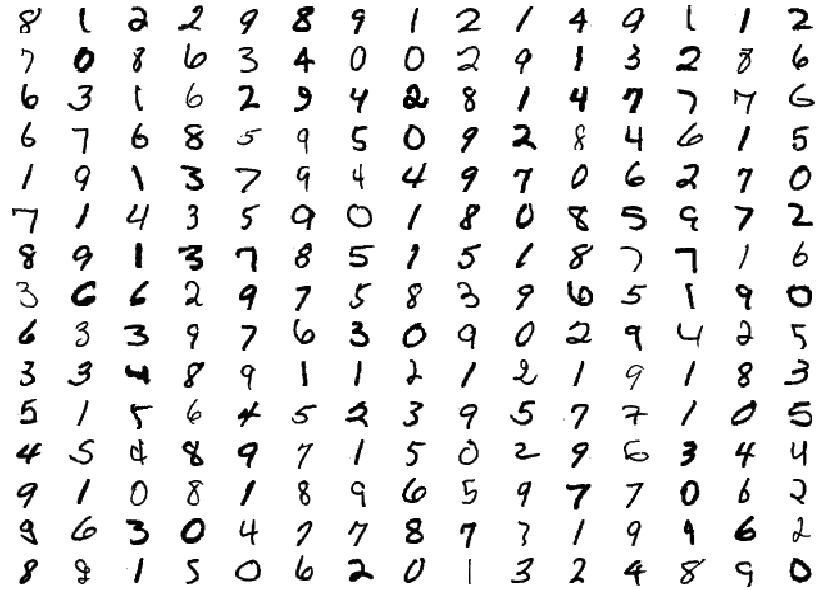
\includegraphics[width=\textwidth]{MNIST_data_examples}
    \caption{Example of 225 randomly chosen digits from the MNIST train set.}
    \label{fig:MNIST_data_examples}
\end{figure}

The MNIST dataset was used in the article \citetitle{Gal2016Active} by \citeauthor{Gal2016Active} to compare the performance of Bayesian CNNs with frequentist CNNs in the context of Active Learning. This experiment was replicated in this work by using the same architecture that was explained in the article.

The experiment consists in starting with a random but balanced sample of 20 images from the MNIST dataset, training a CNN with these images, then take a random sample of 5000 images from the pool set (to save computation time), subsequently computing the probabilities of belonging to each class for each image, afterward acquiring the 10 images that maximize the acquisition function, adding these 10 images to the training set, and repeating this process. In the end, 100 acquisition steps are taken for each acquisition function. This whole process is repeated 3 times with different initial images and the results were averaged.

The acquisition functions used in the original article are the ones mentioned mentioned in chapter \ref{ch:active_learning}, i.e., Bayesian predictive entropy, frequentist predictive entropy, Bayesian variation ratios, frequentist variation ratios, BALD, random, and an additional one called ``Mean STD'' which was not implemented in this work because of its bad performance in the original article.

The architecture of the CNN used was convolution-relu-convolution-relu-max pooling-dropout-dense-relu-dropout-dense-softmax, with 32 convolution kernels, $4 \times 4$ kernel size, $2 \times 2$ pooling, dense layer with 128 units, and dropout probabilities $0.25$ and $0.5$. The CNNs were trained for 50 epochs. For the Bayesian acquisition functions, 100 posterior predictive distribution samples were obtained by using the dropout trick mentioned in chapter \ref{ch:ann}.

The results of the Bayesian and random acquisition functions can be seen in figure \ref{fig:mnist_comparison_active_learning_random}, where the results of our implementation are shown on the left and the original article's results are shown on the right. Our results are very similar with the article's results: apparently, using the variation ratios results in a slightly better performance than BALD or predictive entropy, and more importantly, using the Bayesian acquisition functions results in a much better performance than using a random acquisition function.

\begin{figure}[H]
    \centering
    \subfloat[Our results.]{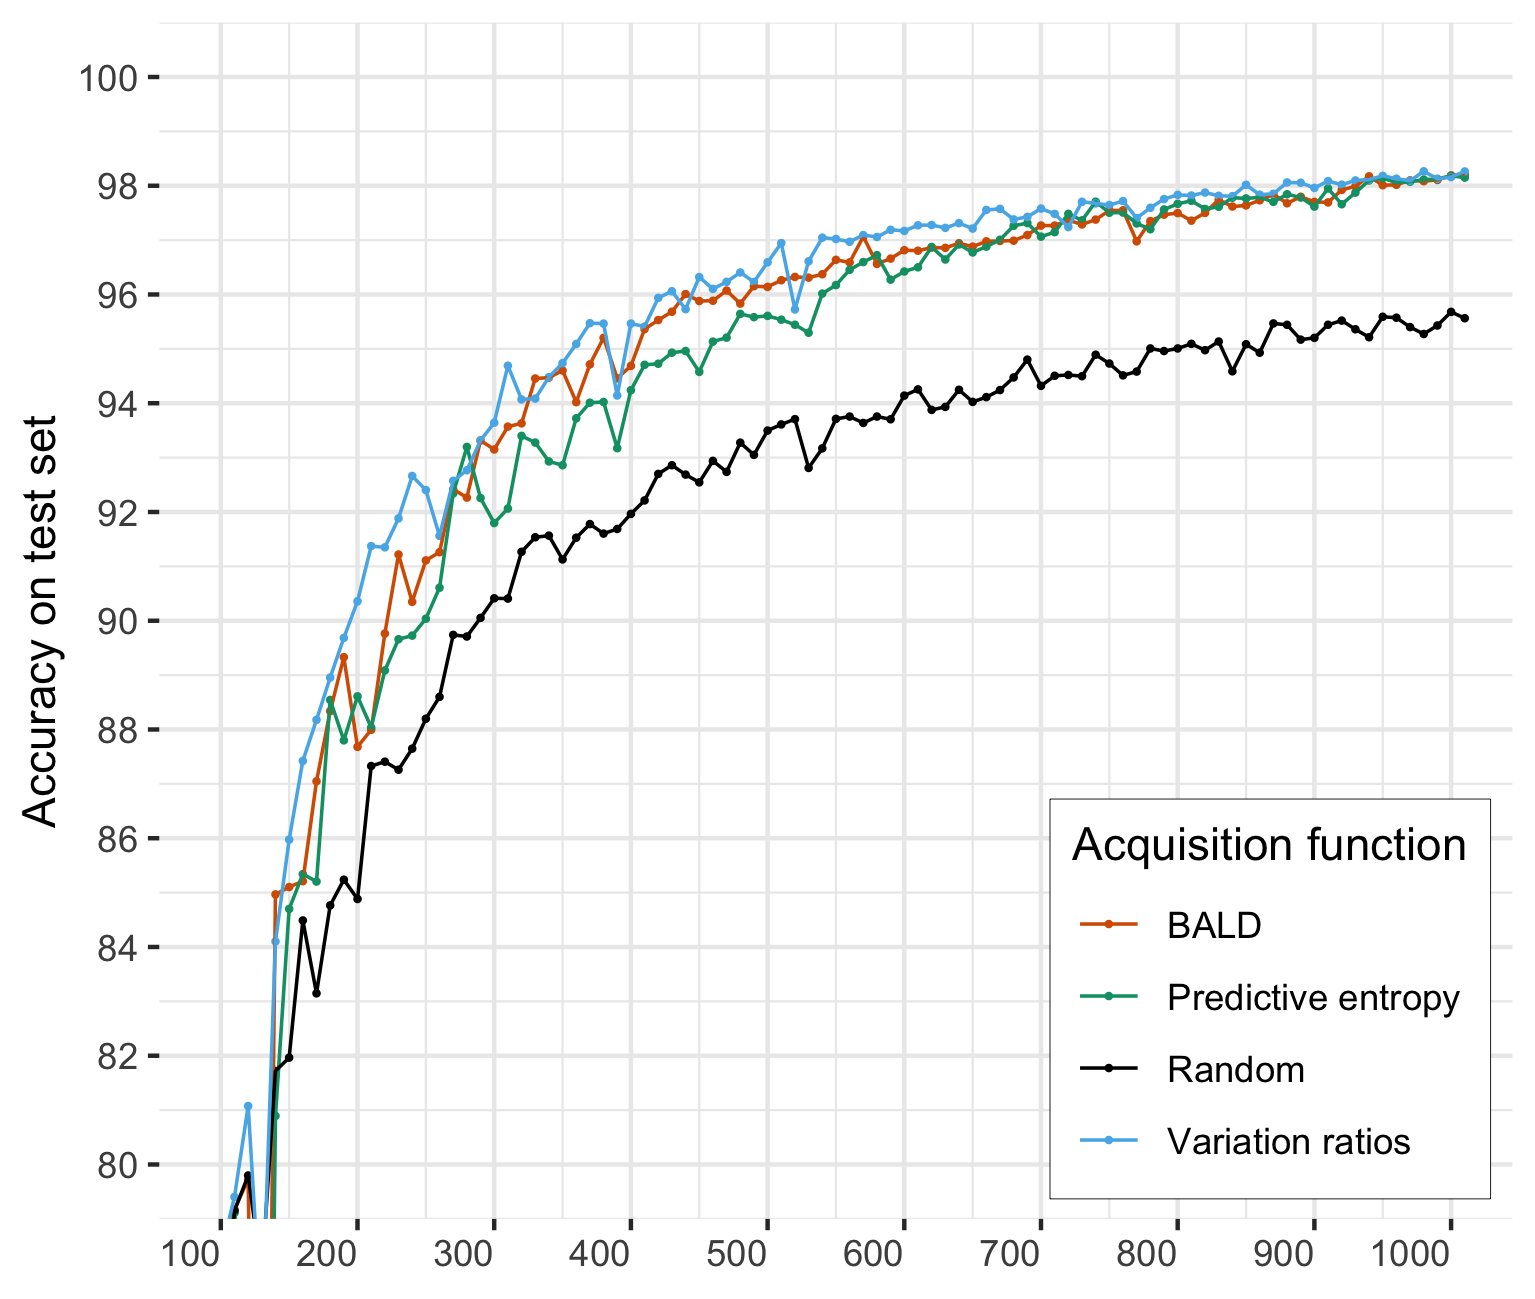
\includegraphics[width=0.5\textwidth]{MNIST_accuracies_bayesian}}
    \hfill
    \subfloat[Paper's results.]{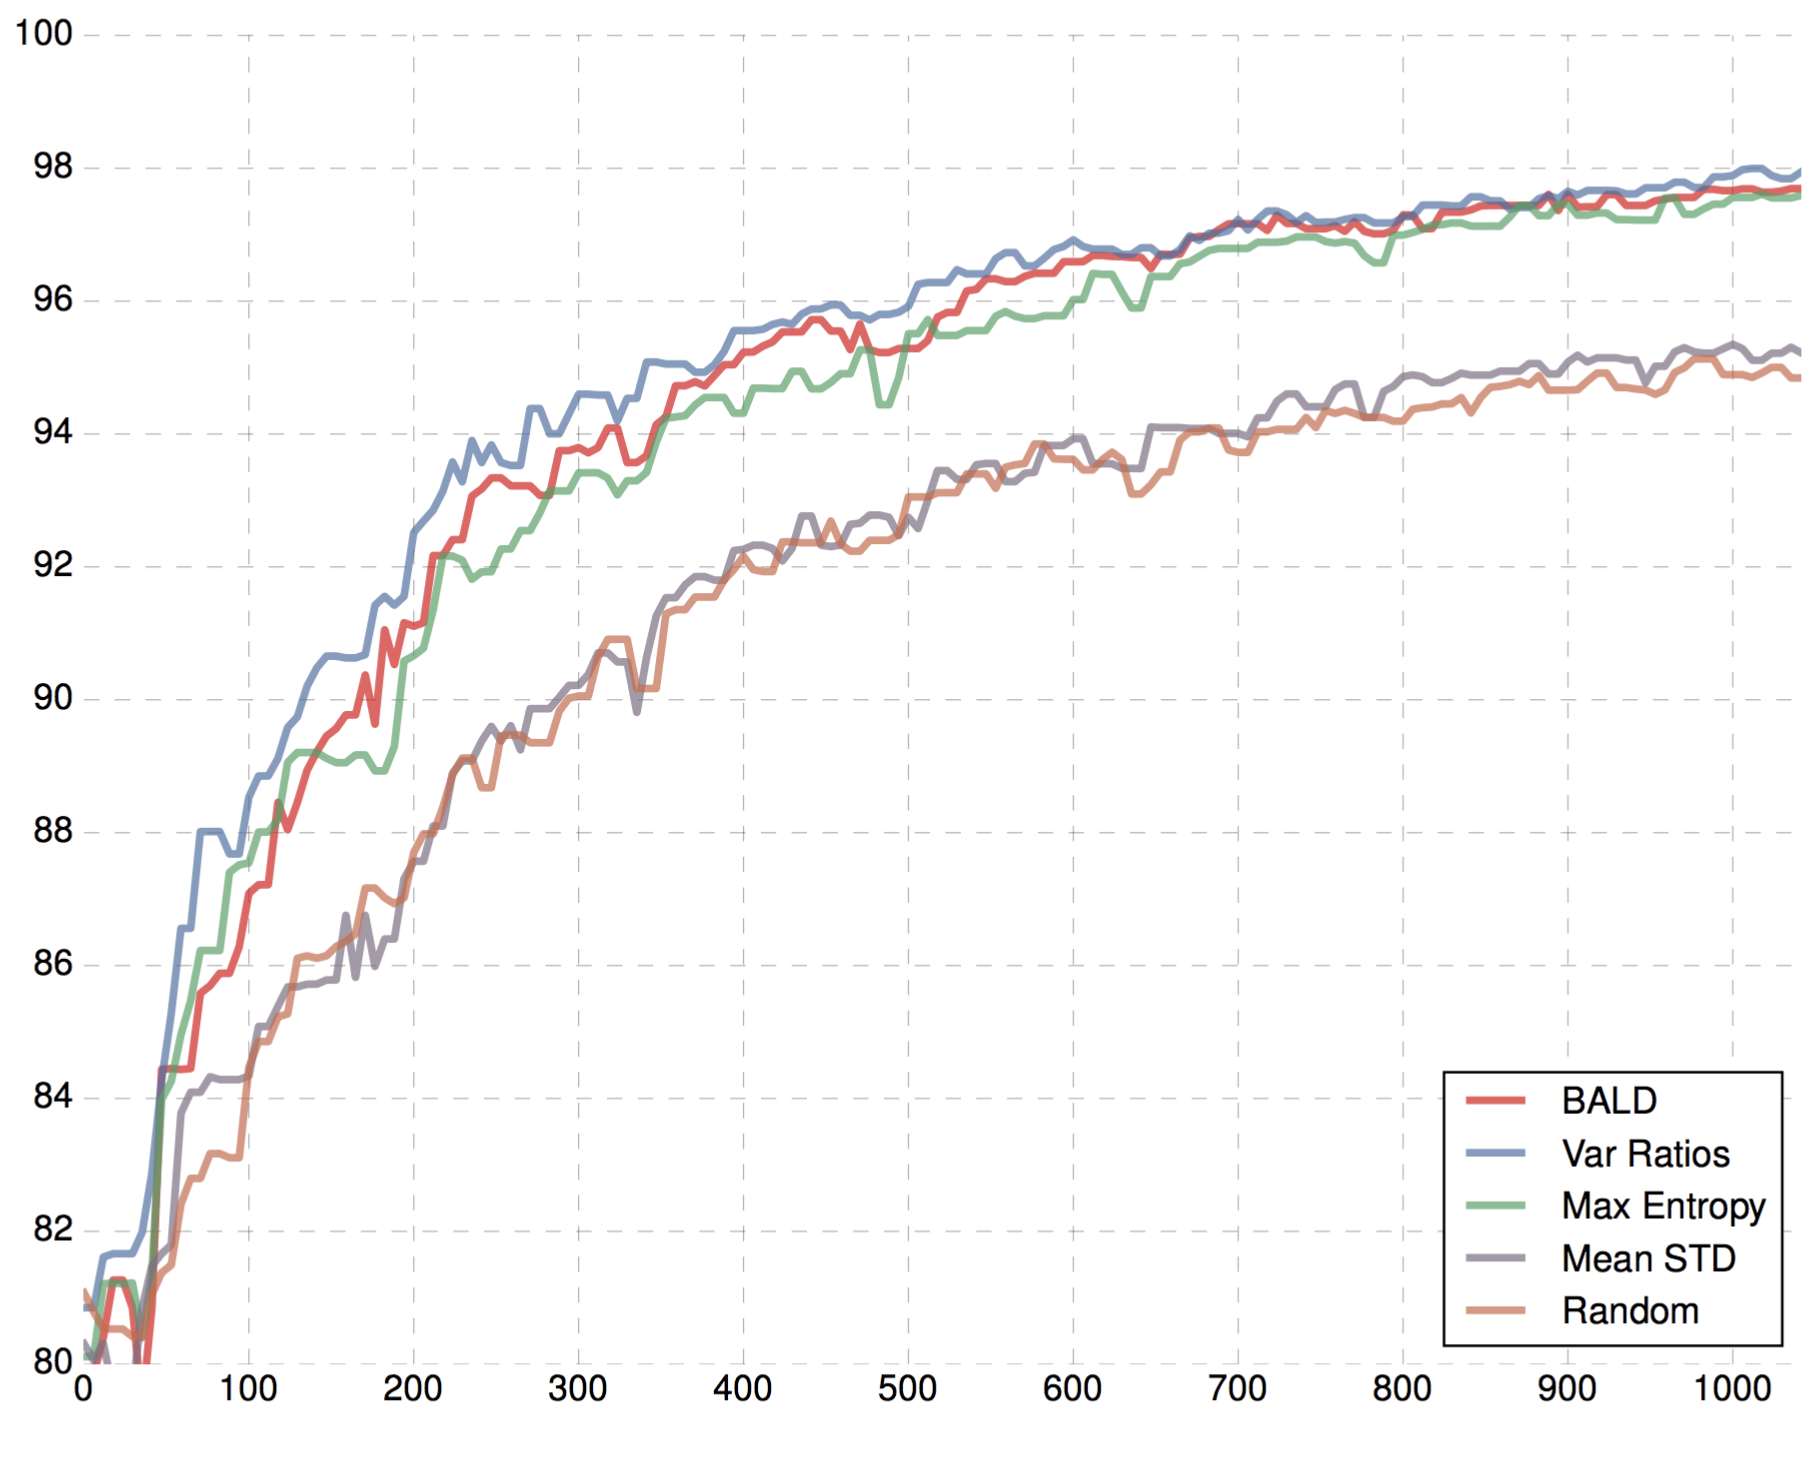
\includegraphics[width=0.5\textwidth]{MNIST_all_gal_islam}}
    \caption{Accuracy of models in each acquisition step. The left picture shows our implementation and the right picture shows \citeauthor{Gal2016Active}'s implementation. The $x$ axis is the number of images.}
    \label{fig:mnist_comparison_active_learning_random}
\end{figure}

Our implementation achieved the goal of outperforming a random acquisition function, however, the results differ when one compares the Bayesian and the frequentist approach. The article's authors claim that the use of a Bayesian approach in the acquisition process of Active Learning leads to better accuracy with fewer images, but in our implementation this does not happen. This can be seen with more detail in figures in \ref{fig:mnist_pred_entropy_AL} and \ref{fig:mnist_var_ratios_AL} that show our results on the left and the article's results on the right. In the article, the frequentist acquisition functions lead to a worse performance than their Bayesian counterparts, while in our implementation there is virtually no distinction.

For example, with predictive entropy in figure \ref{fig:mnist_pred_entropy_AL}, the results seem to be backward and the frequentist acquisition function seems to have a slightly better performance that the Bayesian one. Another difference is that the frequentist acquisition function in the original article achieves a 90\% accuracy with around 300 images, while in our implementation this accuracy is first achieved with around 200 images.

\begin{figure}[H]
  \centering
  \subfloat[Our results.]{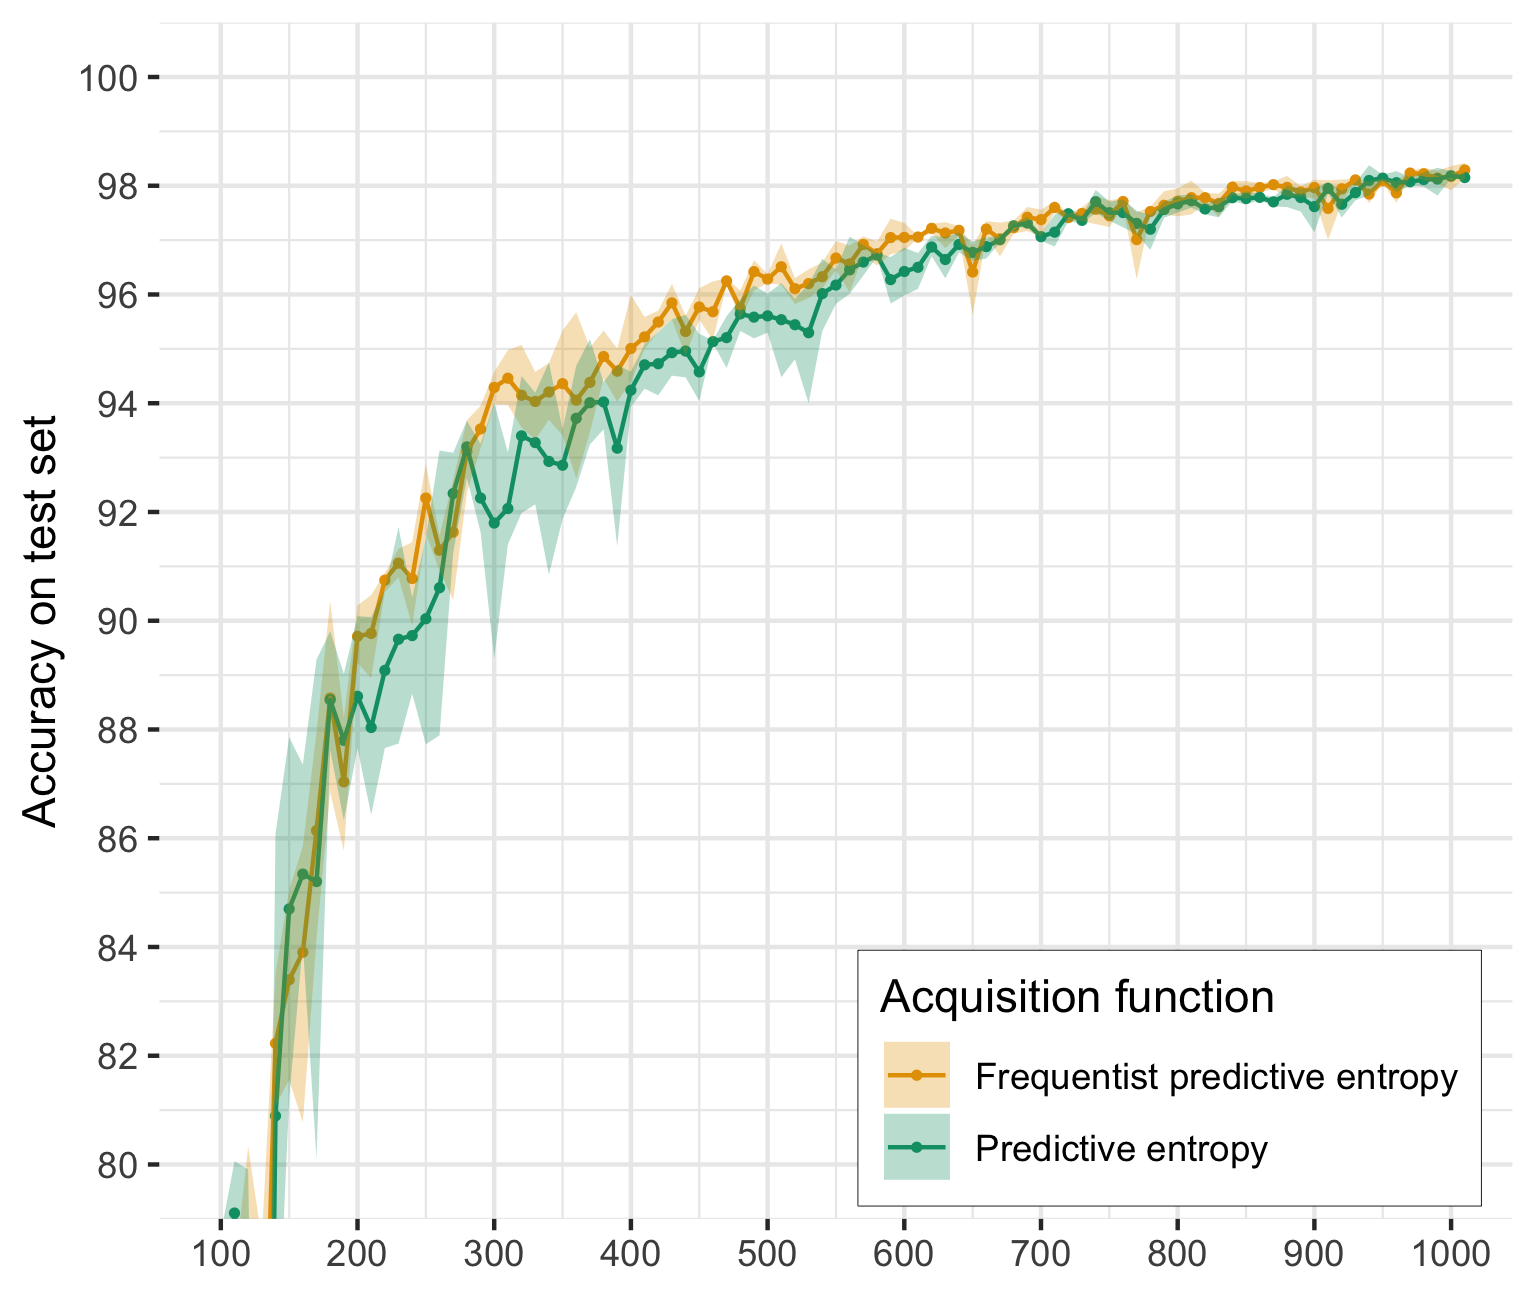
\includegraphics[width=0.5\textwidth]{MNIST_accuracies_pred_ent_ribbon}}
  \hfill
  \subfloat[Paper's results.]{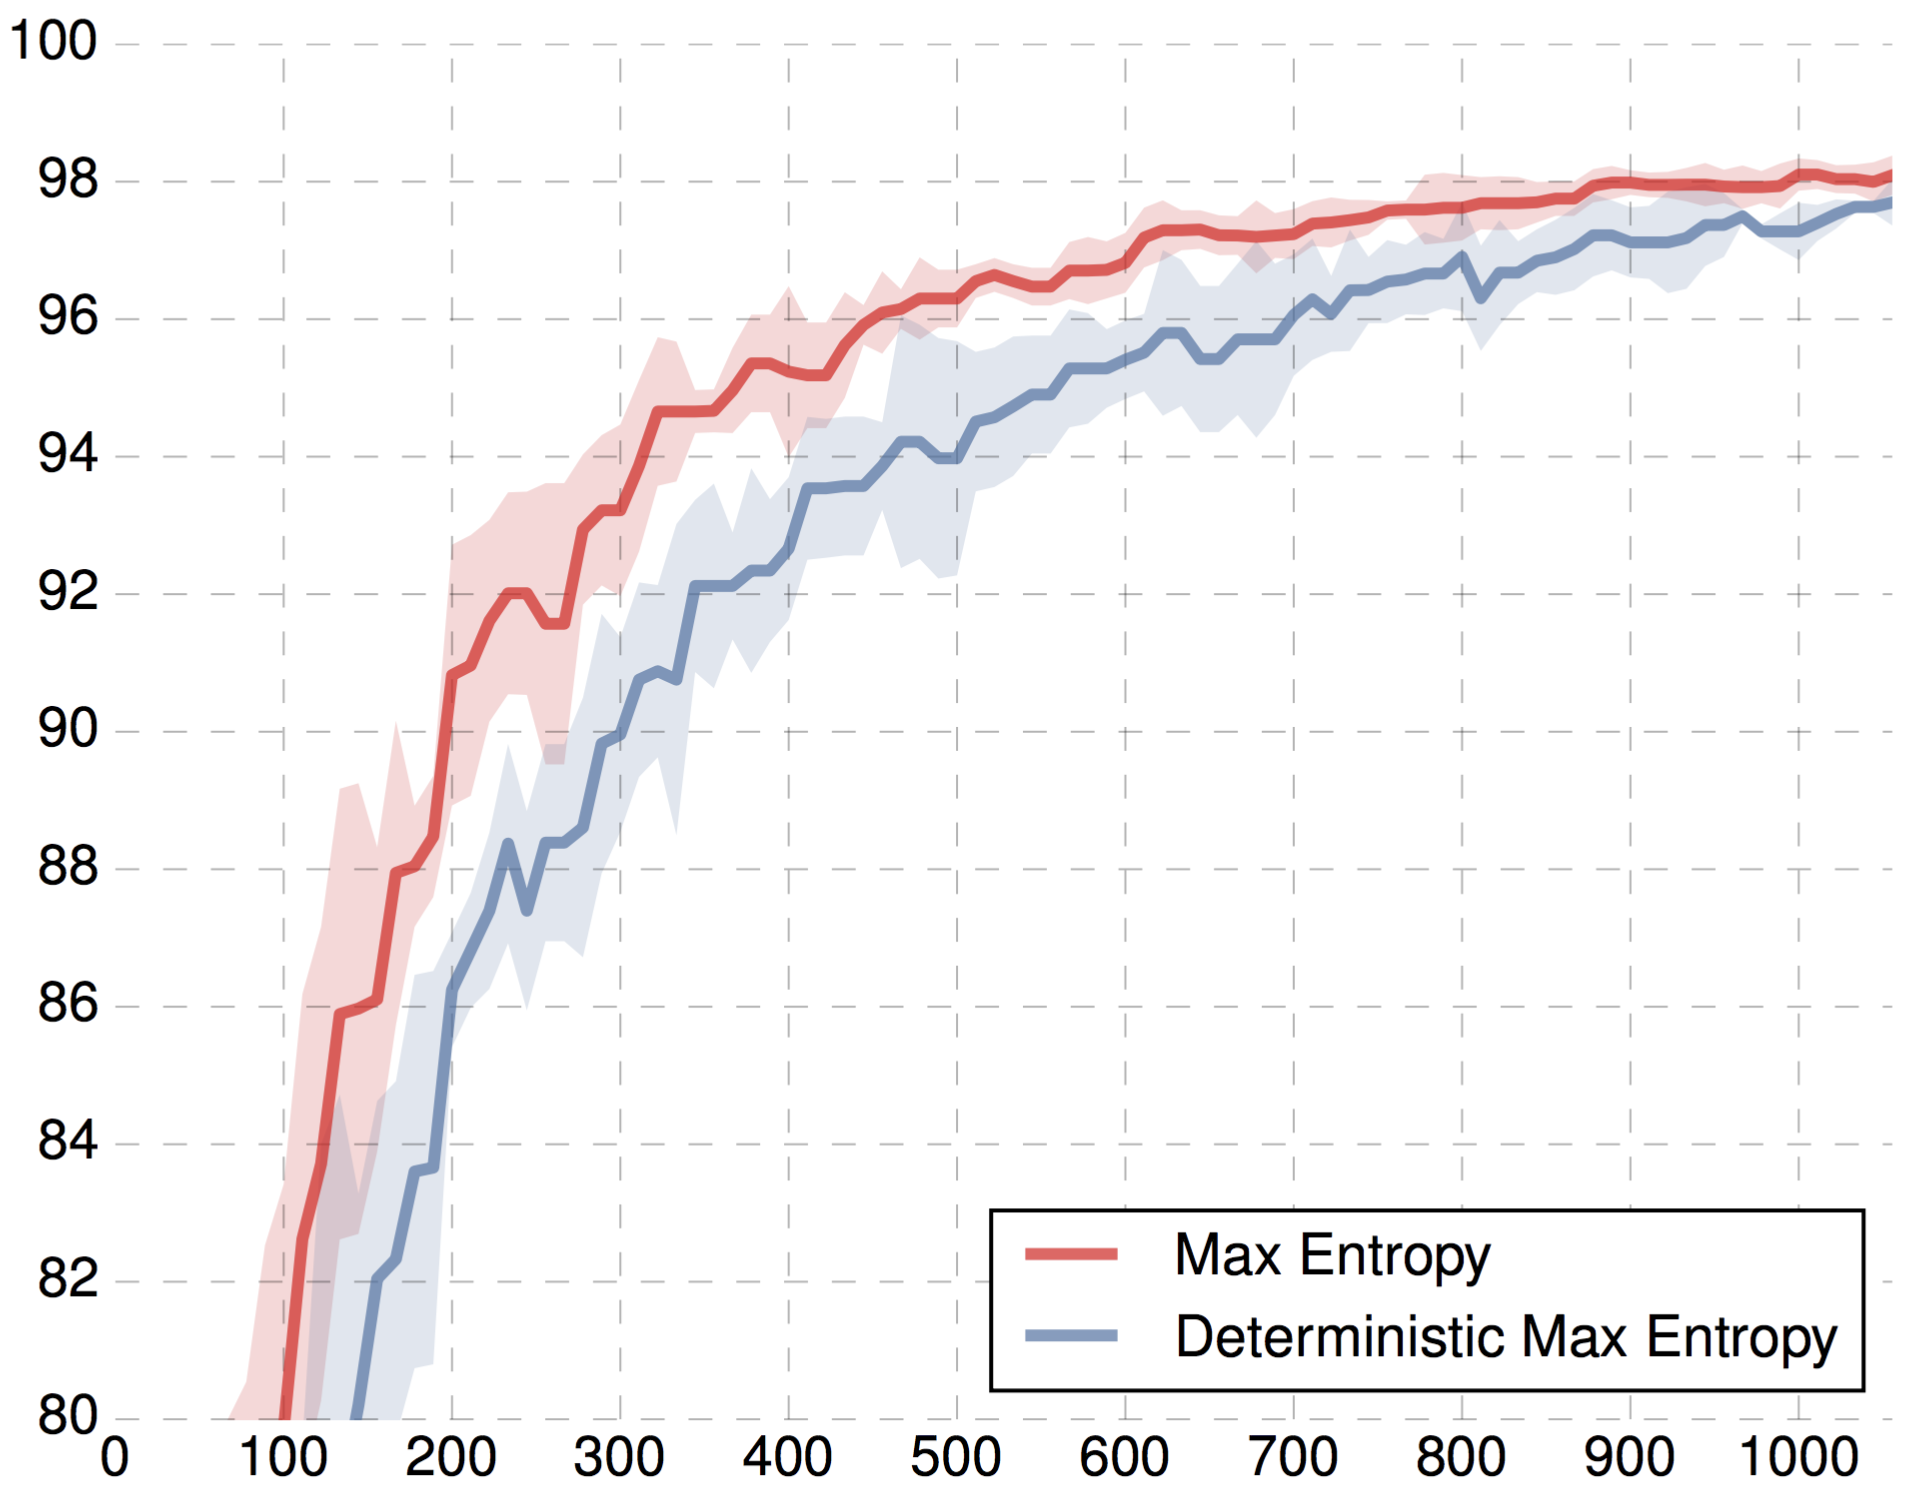
\includegraphics[width=0.5\textwidth]{MNIST_pred_ent_gal_islam}}
  \caption{Accuracy of Bayesian and frequentist models in each acquisition step using predictive entropy as acquisition function. The left picture shows our implementation and the right picture shows \citeauthor{Gal2016Active}'s implementation.}
  \label{fig:mnist_pred_entropy_AL}
\end{figure}

Figure \ref{fig:mnist_var_ratios_AL} shows the results of the variation ratios acquisition functions. While the roles of the frequentist and Bayesian acquisition functions are not reversed as in the previous case, there is apparently no distinction between the two acquisition functions. Moreover, in the original article, a 90\% accuracy is first achieved using the frequentist acquisition function with a little below 300 images, while in our implementation this accuracy is first achieved with around 200 images. Another difference is that with 1000 images and using the frequentist acquisition function, the authors' accuracy is close to 96\%, while in our implementation it is close to 98\%.

\begin{figure}[H]
  \centering
  \subfloat[Our results.]{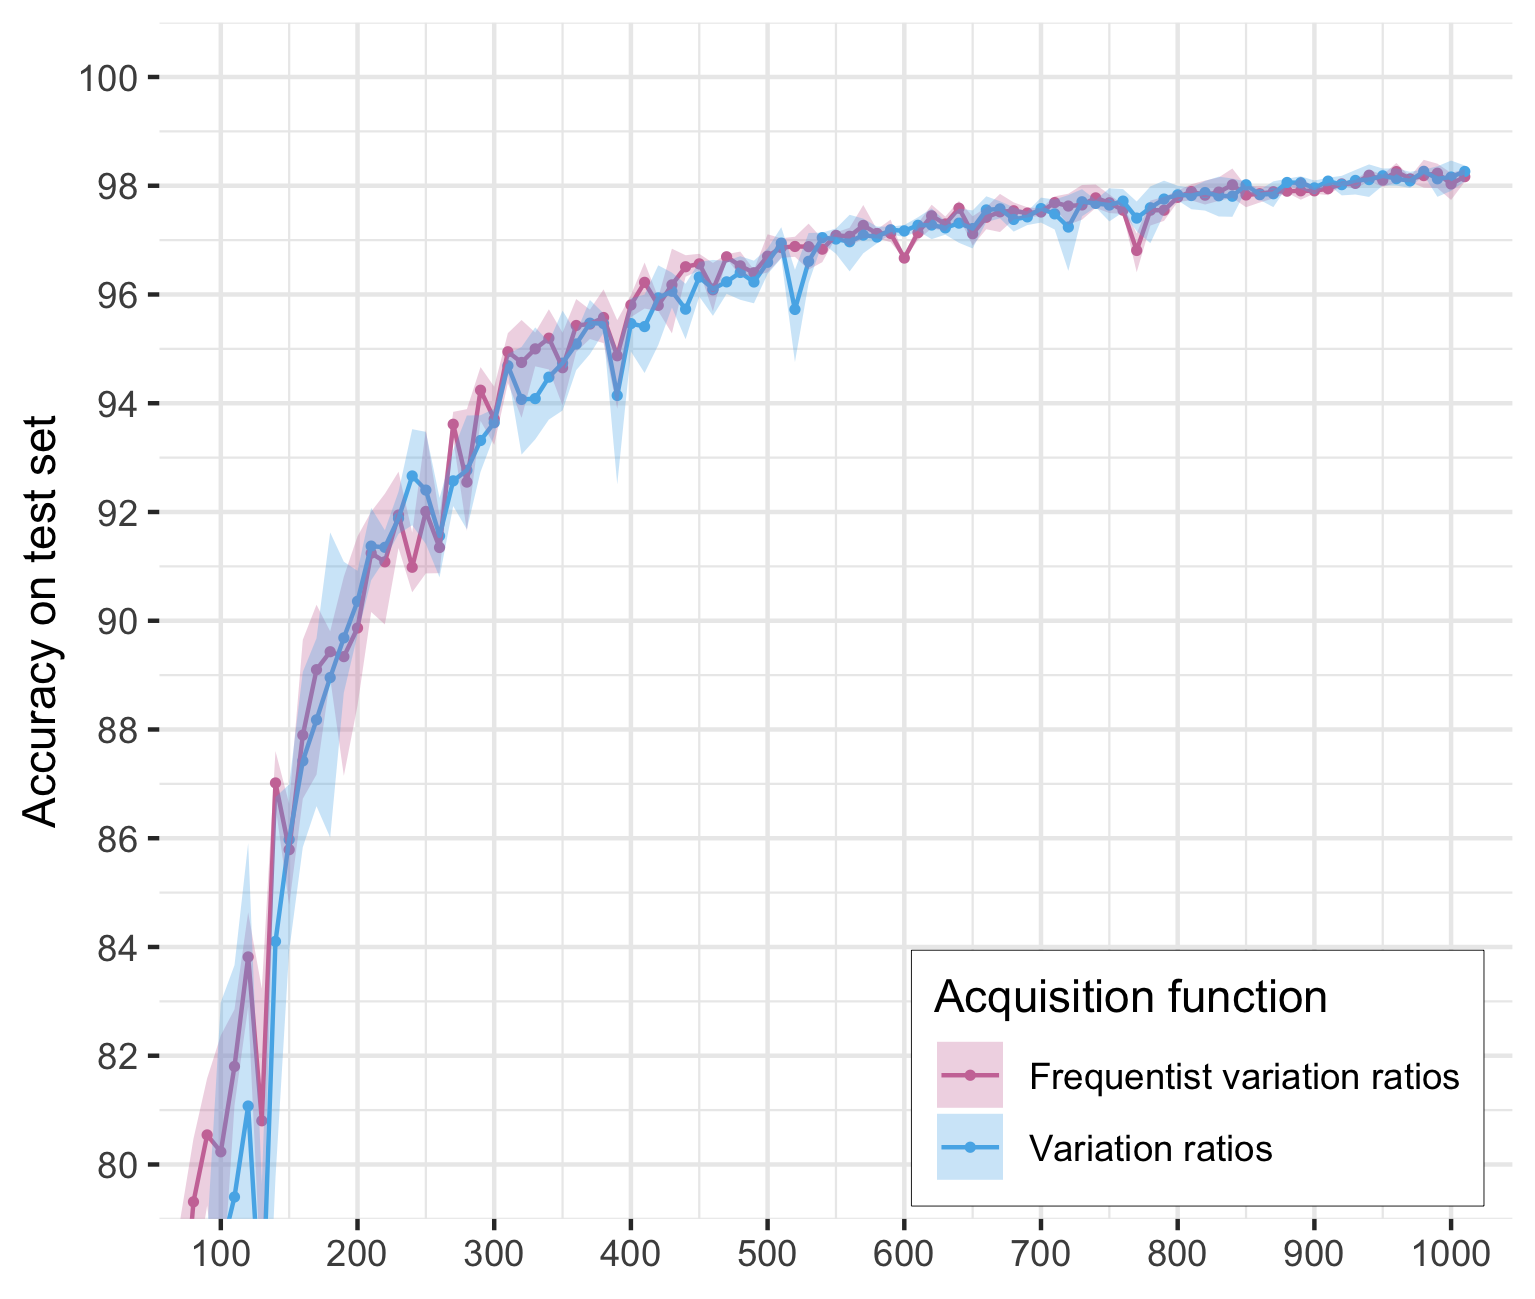
\includegraphics[width=0.5\textwidth]{MNIST_accuracies_var_ratios_ribbon}}
  \hfill
  \subfloat[Paper's results.]{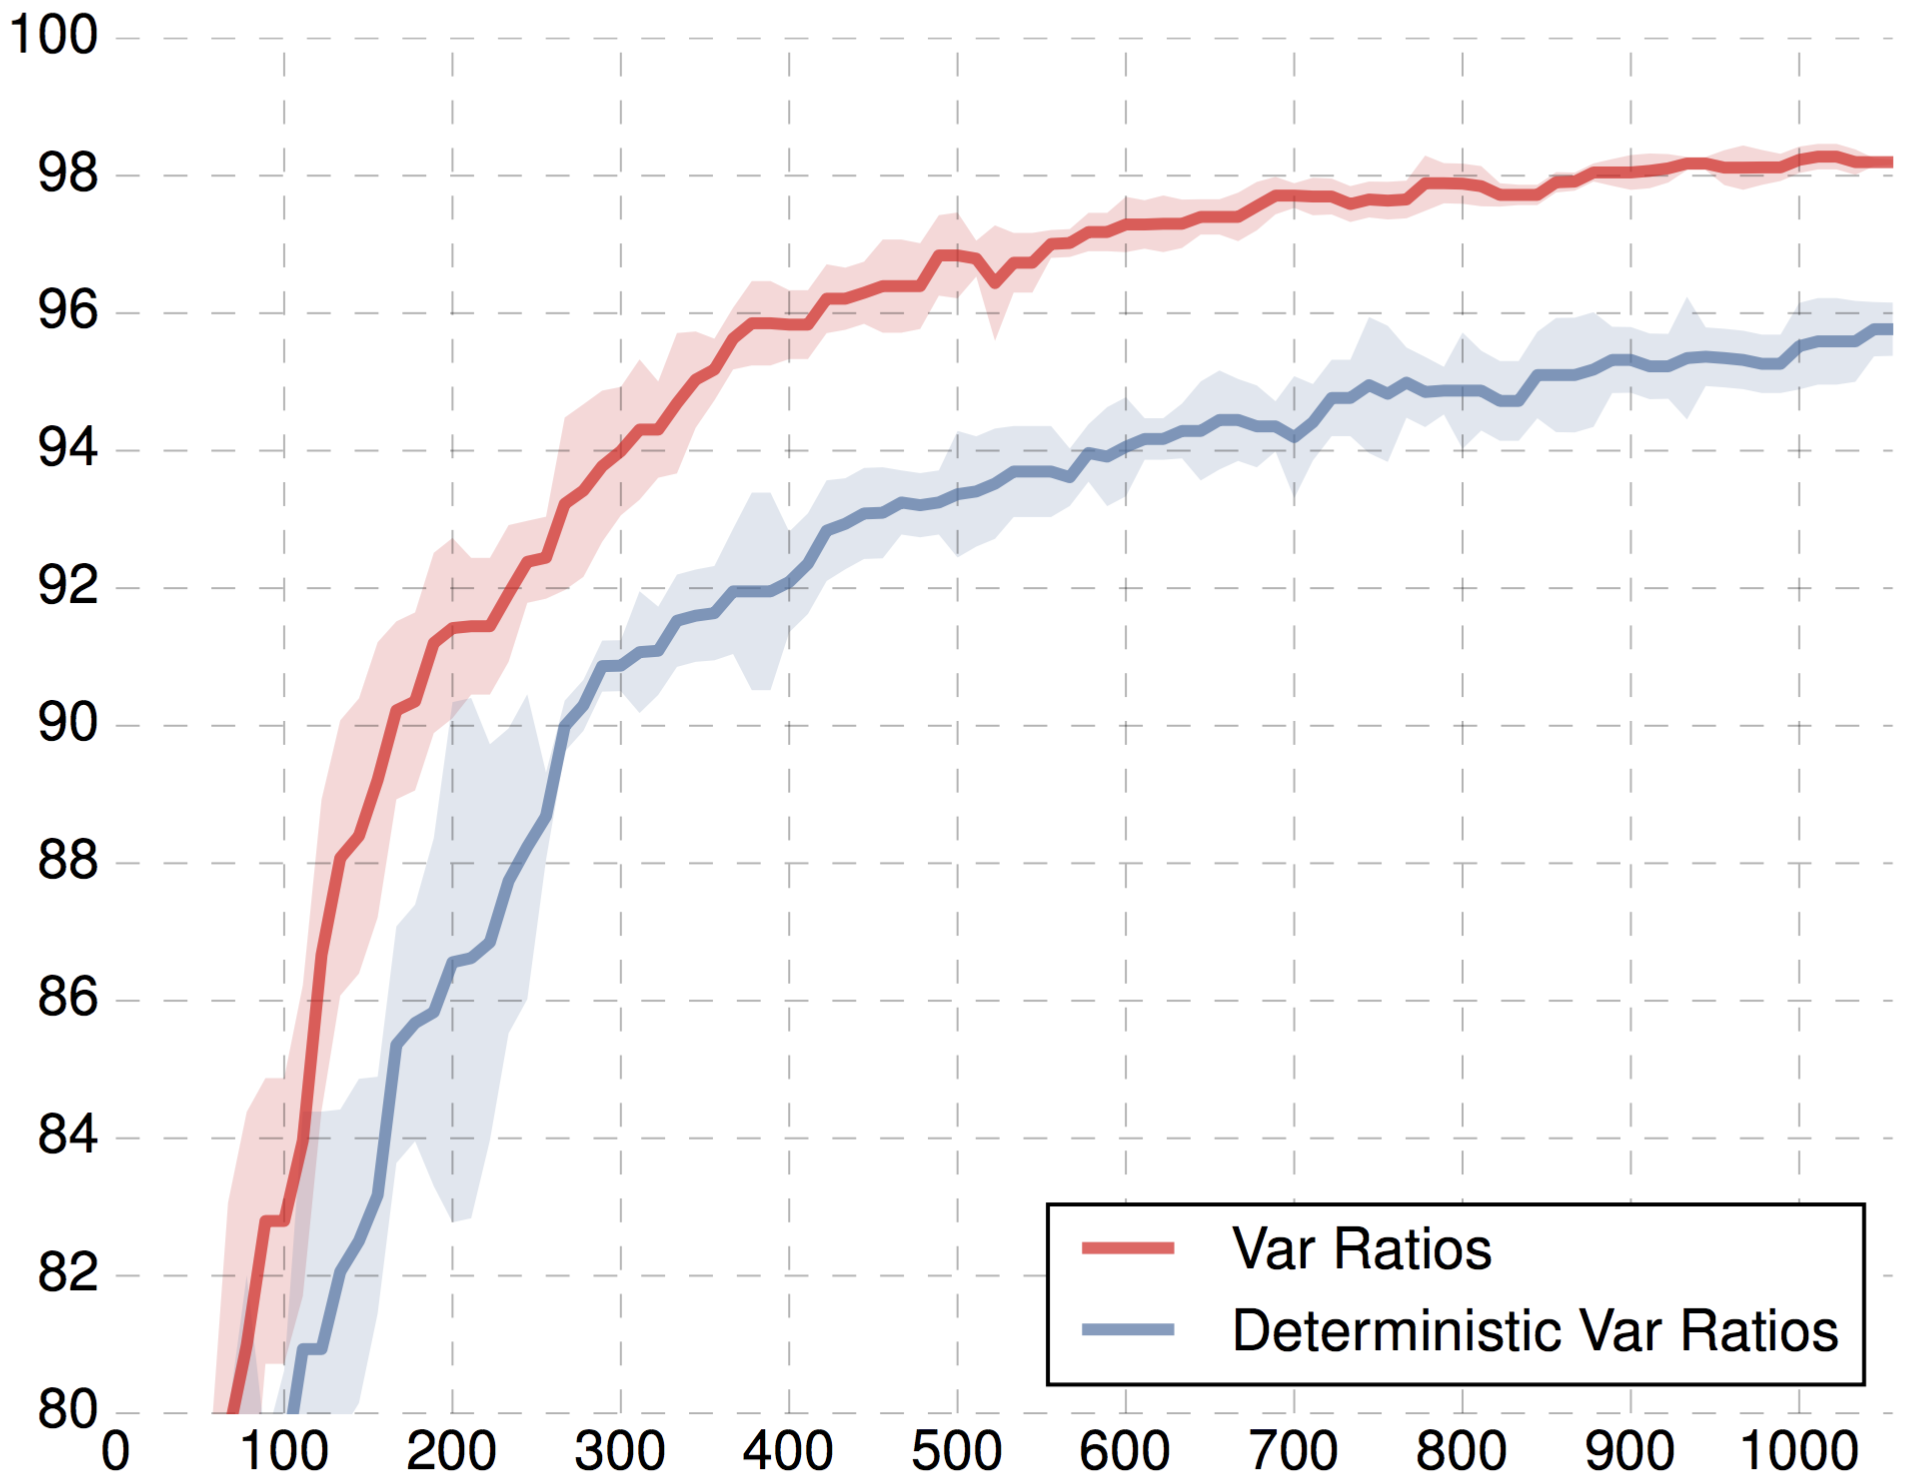
\includegraphics[width=0.5\textwidth]{MNIST_var_ratios_gal_islam}}
  \caption{Accuracy of Bayesian and frequentist models in each acquisition step using variation ratios as acquisition function. The left picture shows our implementation and the right picture shows \citeauthor{Gal2016Active}'s implementation.}
  \label{fig:mnist_var_ratios_AL}
\end{figure}


%%%%%%%%%%%%%%%%%%%%%%%%%%%%%%%%%%%%%%%%%%%%%%%%%%%%%%%%%%%%%%
%%%%%%%%%%%%%%%%%%%%%%%%%%%%%%%%%%%%%%%%%%%%%%%%%%%%%%%%%%%%%%
\section{Cats and dogs dataset}
%%%%%%%%%%%%%%%%%%%%%%%%%%%%%%%%%%%%%%%%%%%%%%%%%%%%%%%%%%%%%%
%%%%%%%%%%%%%%%%%%%%%%%%%%%%%%%%%%%%%%%%%%%%%%%%%%%%%%%%%%%%%%

The cats and dogs dataset was first used for a CAPTCHA developed by Microsoft Research called Asirra \cite{elson2007asirra}. It is a collection of \numprint{25000} pictures of size $64 \times 64$, of which half are cats and half are dogs. Figure \ref{fig:cats_dogs_data_examples} shows 30 randomly chosen cats and 30 randomly chosen dogs from the training set.

\begin{figure}[ht]
    \centering
    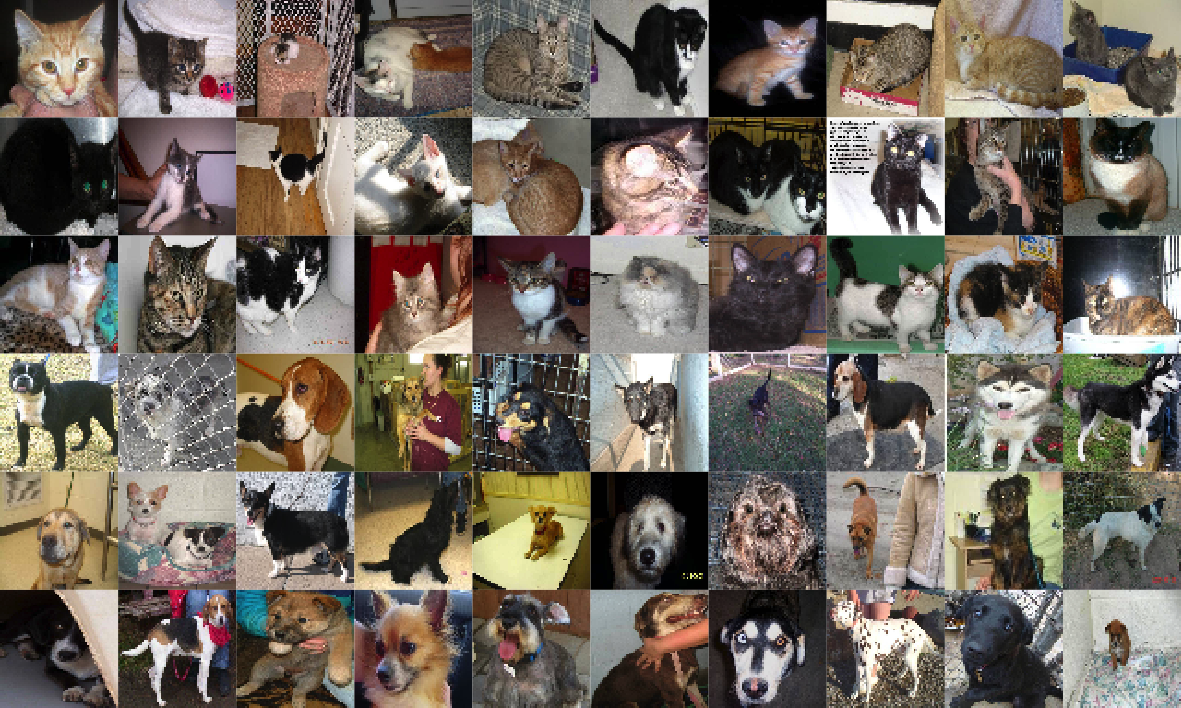
\includegraphics[width=\textwidth]{cats_dogs_data_examples}
    \caption{Example of 60 randomly chosen cats and 30 randomly chosen dogs from the dataset.}
    \label{fig:cats_dogs_data_examples}
\end{figure}

The process of this experiment is very similar to the one followed in the MNIST dataset. First, a balanced set of 100 images was randomly chosen and used to train a first model. Then a random sample of 2000 images was chosen from the pool set, from which the predicted probabilities of belonging to each class were computed, subsequently the 50 images with the highest acquisition function value were chosen and added to the training set. The final number of acquisition steps was 50 and, once more, the whole process was repeated 3 times with different initial images.

The architecture used was convolution-relu-convolution-relu-max pooling-dropout-convolution-relu-max pooling-dropout-dense-relu-dropout-dense-softmax with 32 convolution kernels, $3 \times 3$ kernel size, $2 \times 2$ pooling, dense layer with 64 units, and dropout probabilities $0.25$, $0.25$ and $0.5$. The CNNs were trained for 200 epochs. Once more, for the Bayesian acquisition functions 100 posterior predictive distribution samples were obtained by using the dropout trick.

The results of the Bayesian and random acquisition functions can be seen in figure \ref{fig:cats_dogs_accuracies_bayesian}. In this case, it is difficult to say that using any of the Bayesian acquisition functions results in a better performance than using a random acquisition function. In the last steps it is clear that the variation ratios acquisition function results in a better accuracy, but the difference is not as abrupt as it was in the MNIST dataset.

\begin{figure}[H]
    \centering
    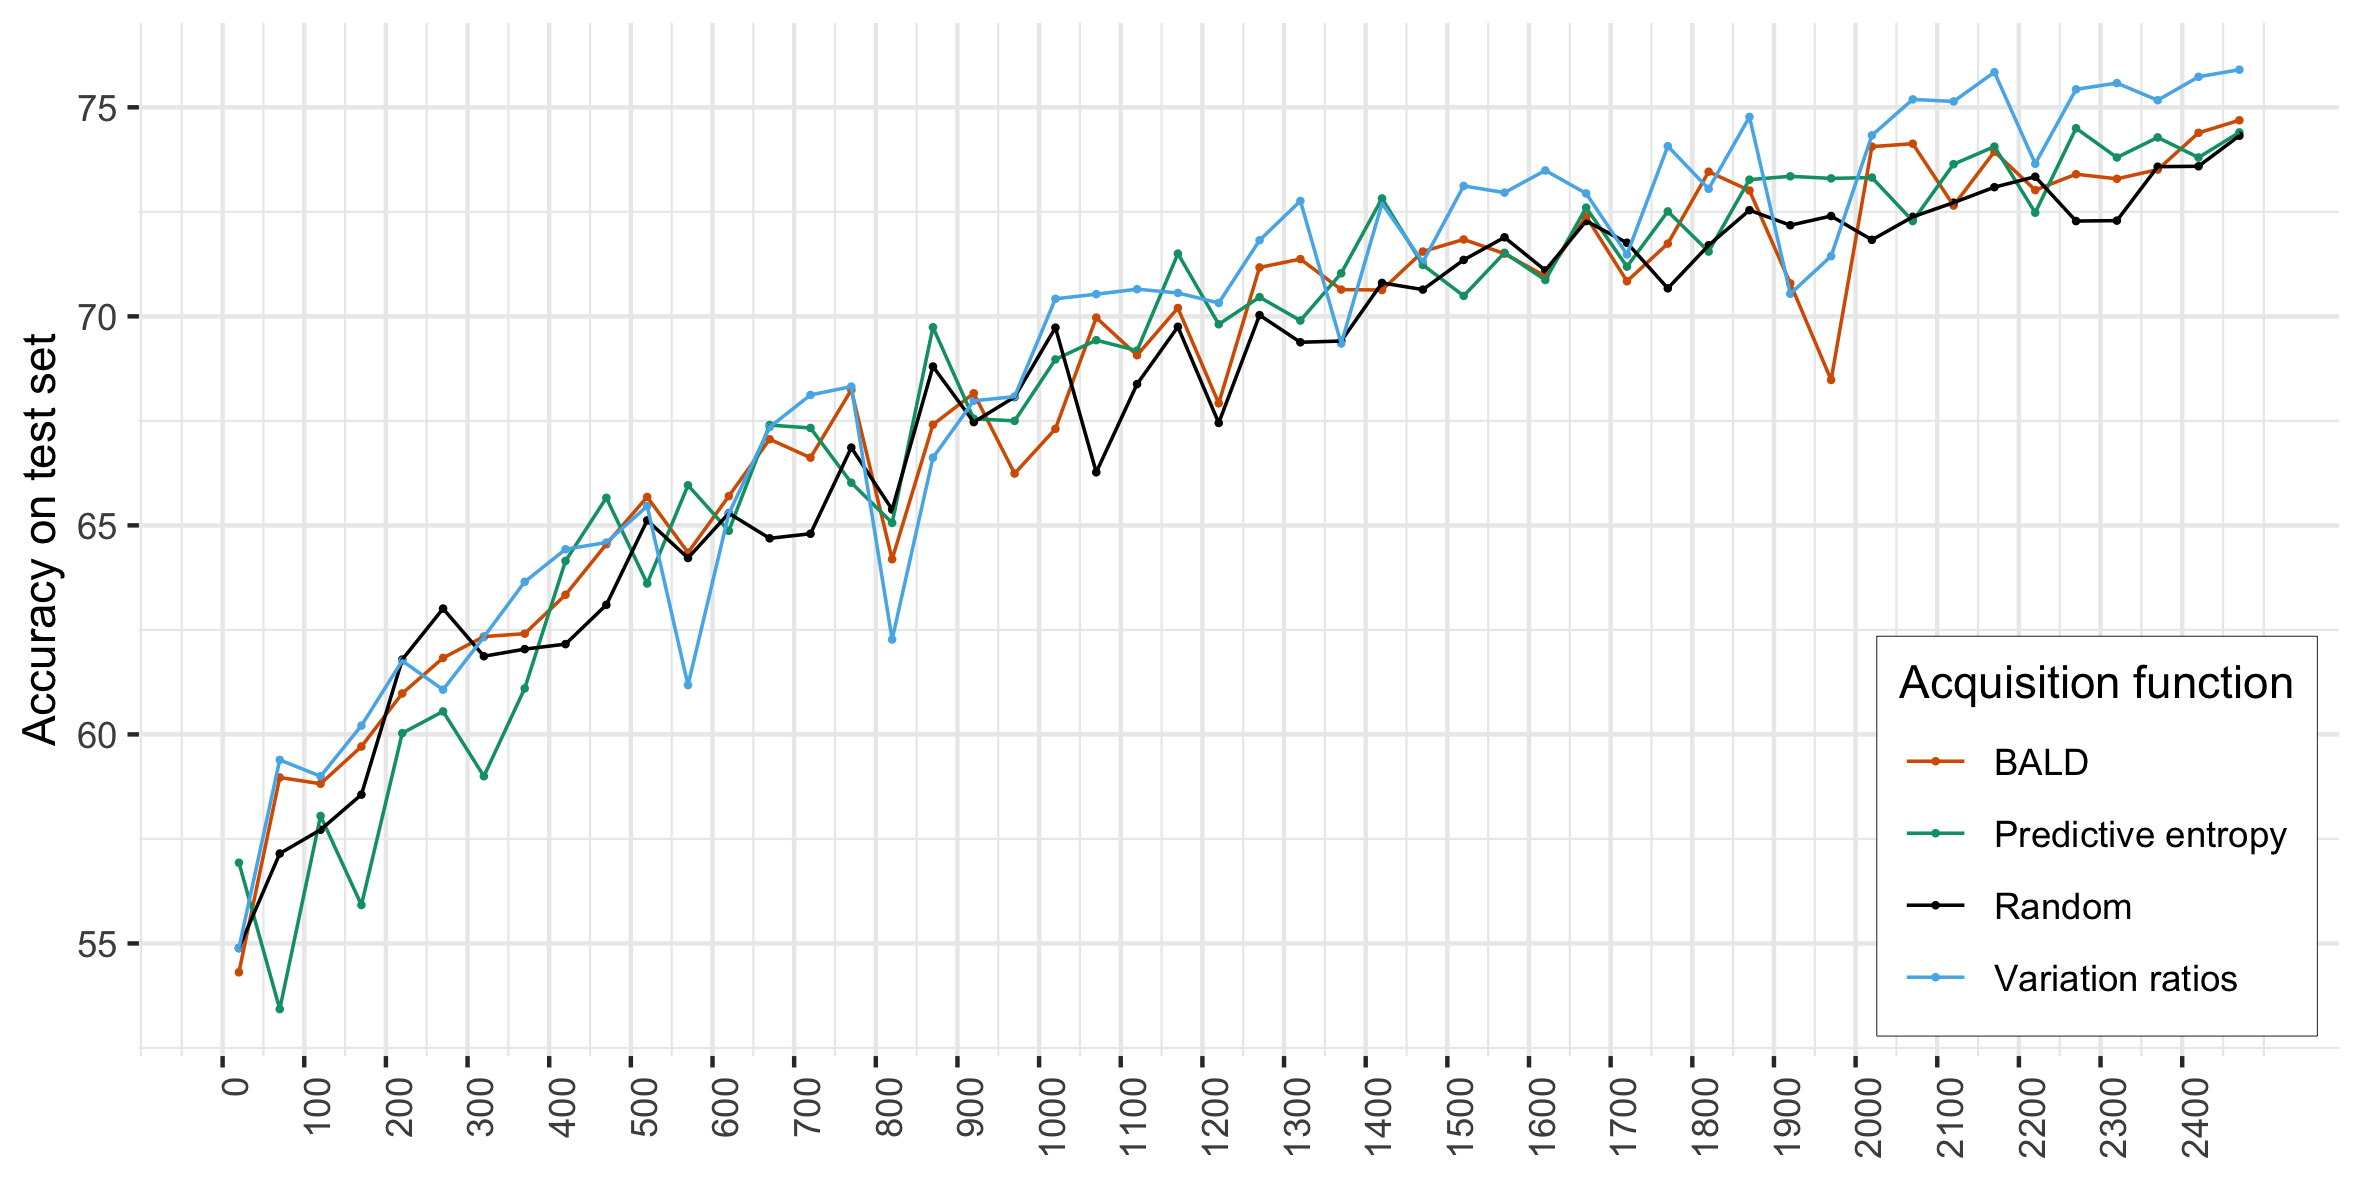
\includegraphics[width=\textwidth]{cats_dogs_accuracies_bayesian}
    \caption{Accuracy of models in each acquisition step in the cats and dogs dataset.}
    \label{fig:cats_dogs_accuracies_bayesian}
\end{figure}

Figure \ref{fig:cats_dogs_bayesian_vs_freq} shows the comparison of the frequentist and Bayesian acquisition functions, with predictive entropy on the left and variation ratios on the right. As with the MNIST dataset, there is no clear distinction between the frequentist and the Bayesian acquisition functions.

\begin{figure}[H]
    \centering
    \subfloat[Predictive entropy.]{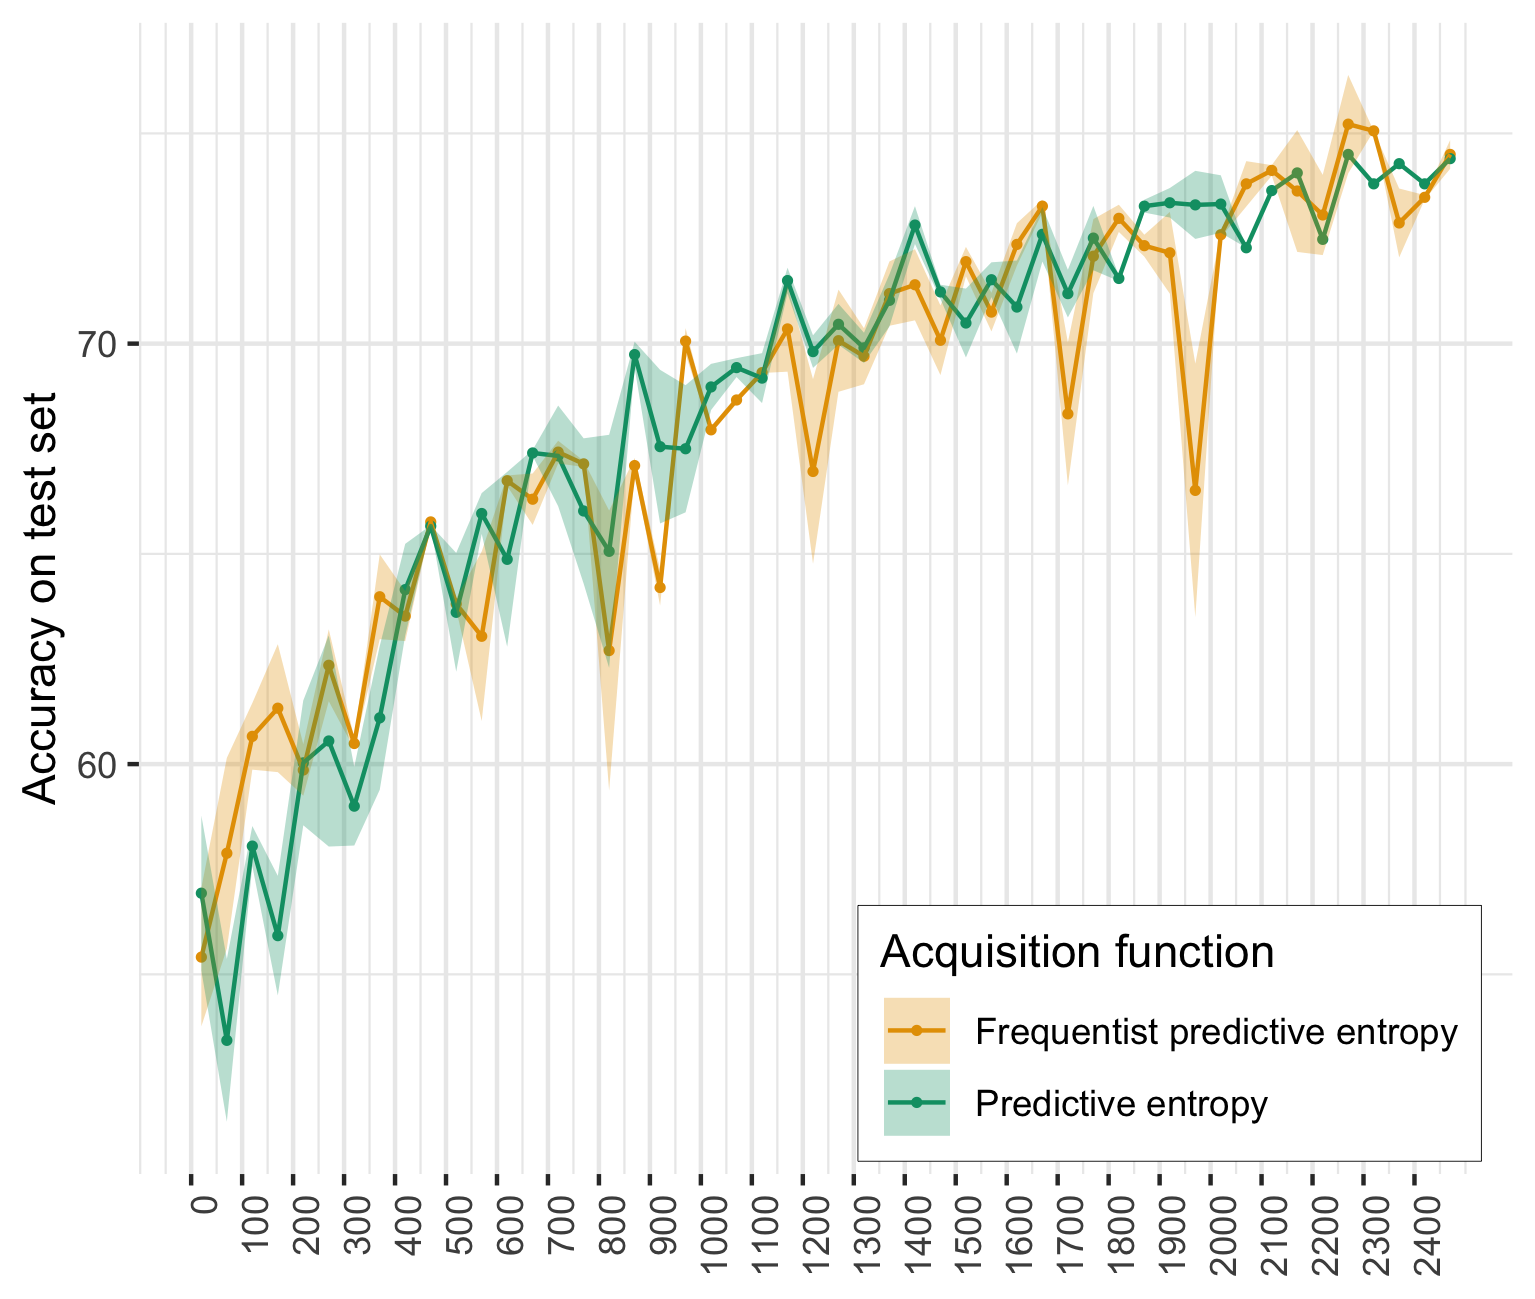
\includegraphics[width=0.5\textwidth]{cats_dogs_accuracies_pred_ent_ribbon}}
    \hfill
    \subfloat[Variation ratios.]{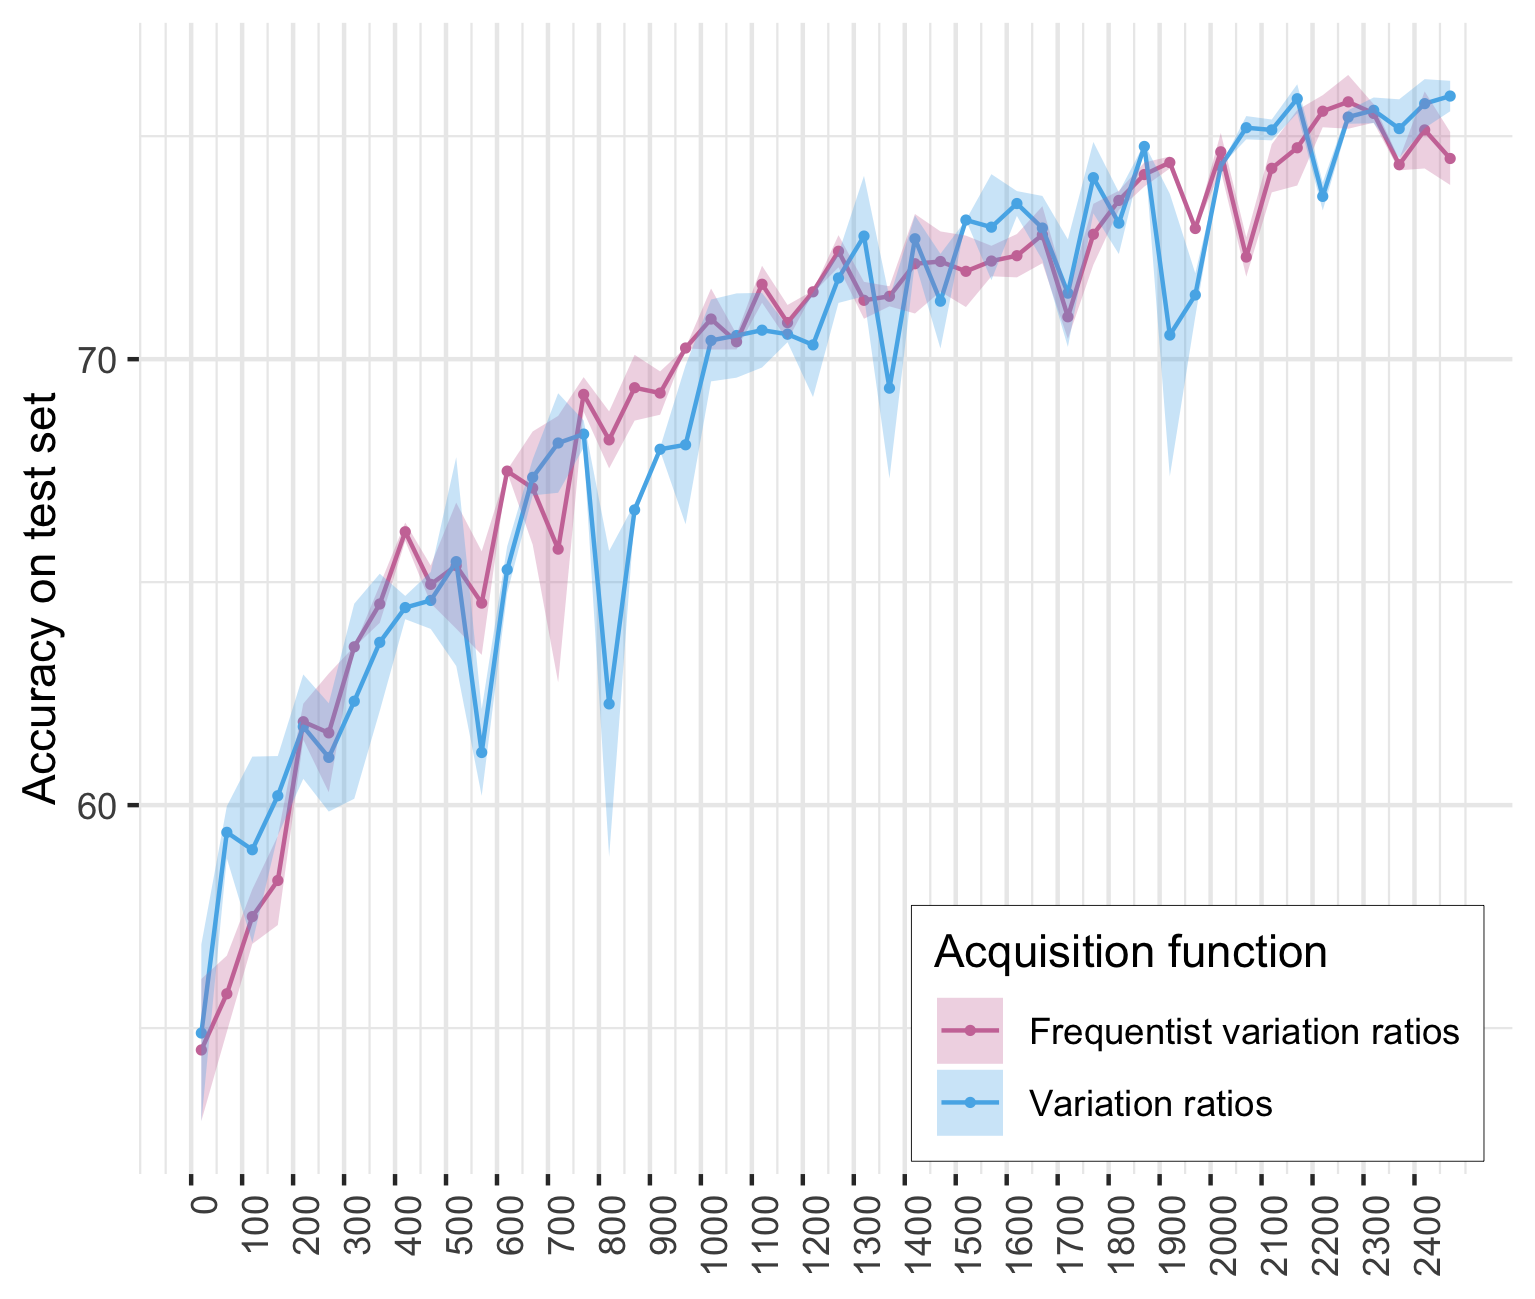
\includegraphics[width=0.5\textwidth]{cats_dogs_accuracies_var_ratios_ribbon}}
    \caption{Accuracy of models in each acquisition step.}
    \label{fig:cats_dogs_bayesian_vs_freq}
\end{figure}




%%%%%%%%%%%%%%%%%%%%%%%%%%%%%%%%%%%%%%%%%%%%%%%%%%%%%%%%%%%%%%
%%%%%%%%%%%%%%%%%%%%%%%%%%%%%%%%%%%%%%%%%%%%%%%%%%%%%%%%%%%%%%
\section{CIFAR-10 dataset}
%%%%%%%%%%%%%%%%%%%%%%%%%%%%%%%%%%%%%%%%%%%%%%%%%%%%%%%%%%%%%%
%%%%%%%%%%%%%%%%%%%%%%%%%%%%%%%%%%%%%%%%%%%%%%%%%%%%%%%%%%%%%%

The CIFAR10 was introduced in \citeyear{krizhevsky2009learning}, and the name comes from the Canadian Institute for Advanced Research, who funded the project in which it was first used \cite{krizhevsky2009learning}. It consists of \numprint{60000} color images of size $32 \times 32$ representing 10 different types of objects, these being \textit{airplane}, \textit{automobile}, \textit{bird}, \textit{cat}, \textit{deer}, \textit{dog}, \textit{frog}, \textit{horse}, \textit{ship} and \textit{truck}. The classes are balanced in the dataset, meaning that each class has the same number of images. Of the \numprint{60000} images, \numprint{50000} are used as a training set and the rest as test set. The training set and the test are also balanced. Figure \ref{fig:CIFAR10_data_examples} shows 200 randomly chosen images from the training set.


\begin{figure}[H]
    \centering
    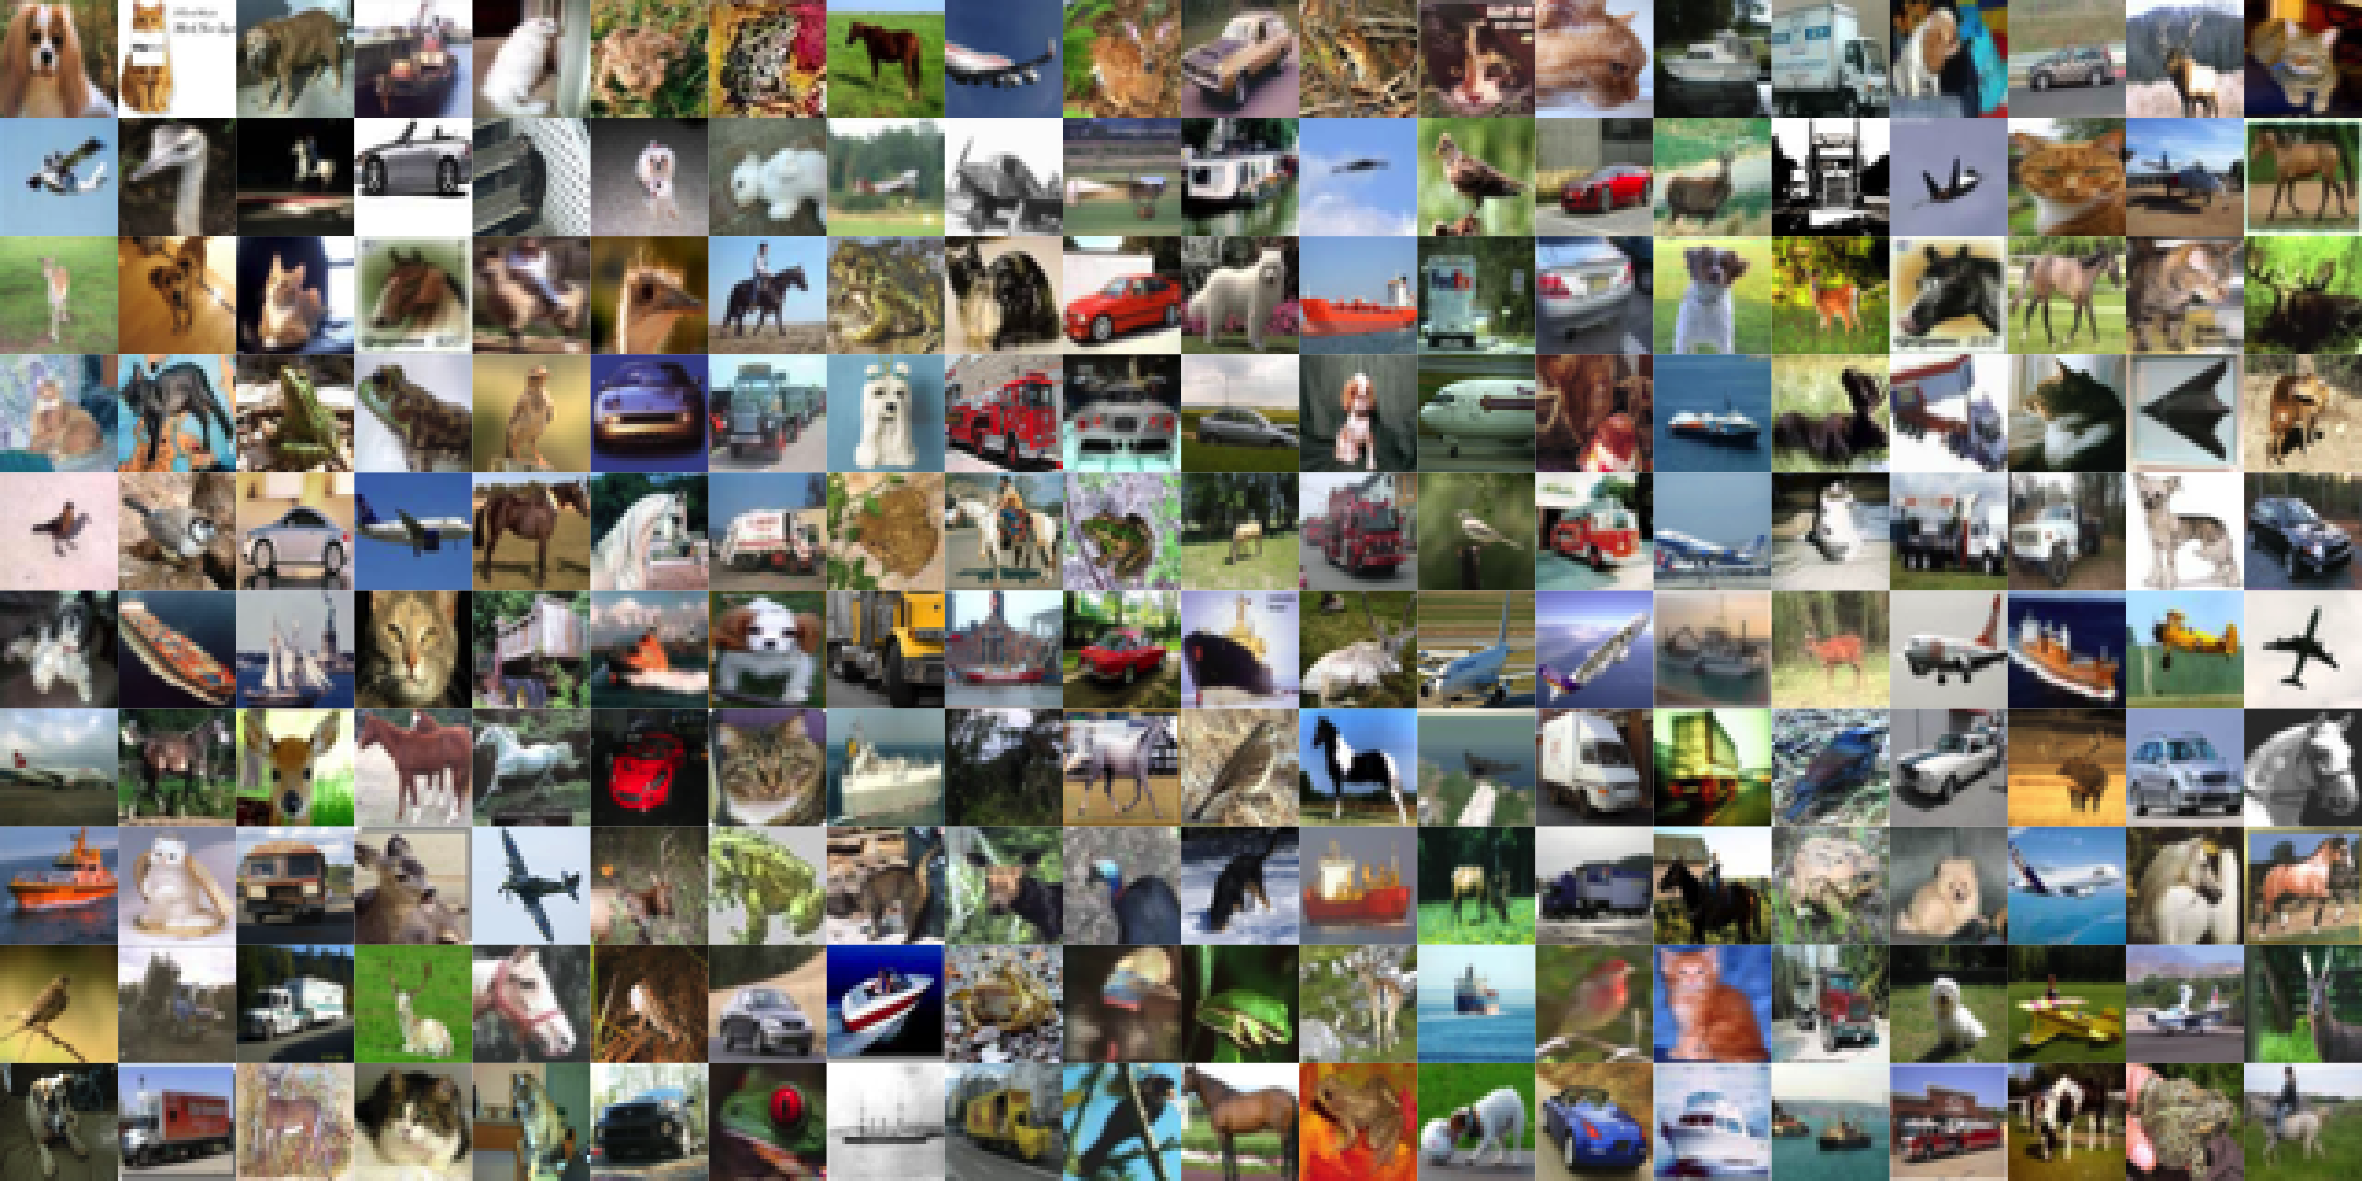
\includegraphics[width=\textwidth]{CIFAR10_data_examples}
    \caption{Example of 200 randomly chosen images from the dataset.}
    \label{fig:CIFAR10_data_examples}
\end{figure}


\begin{figure}[H]
    \centering
    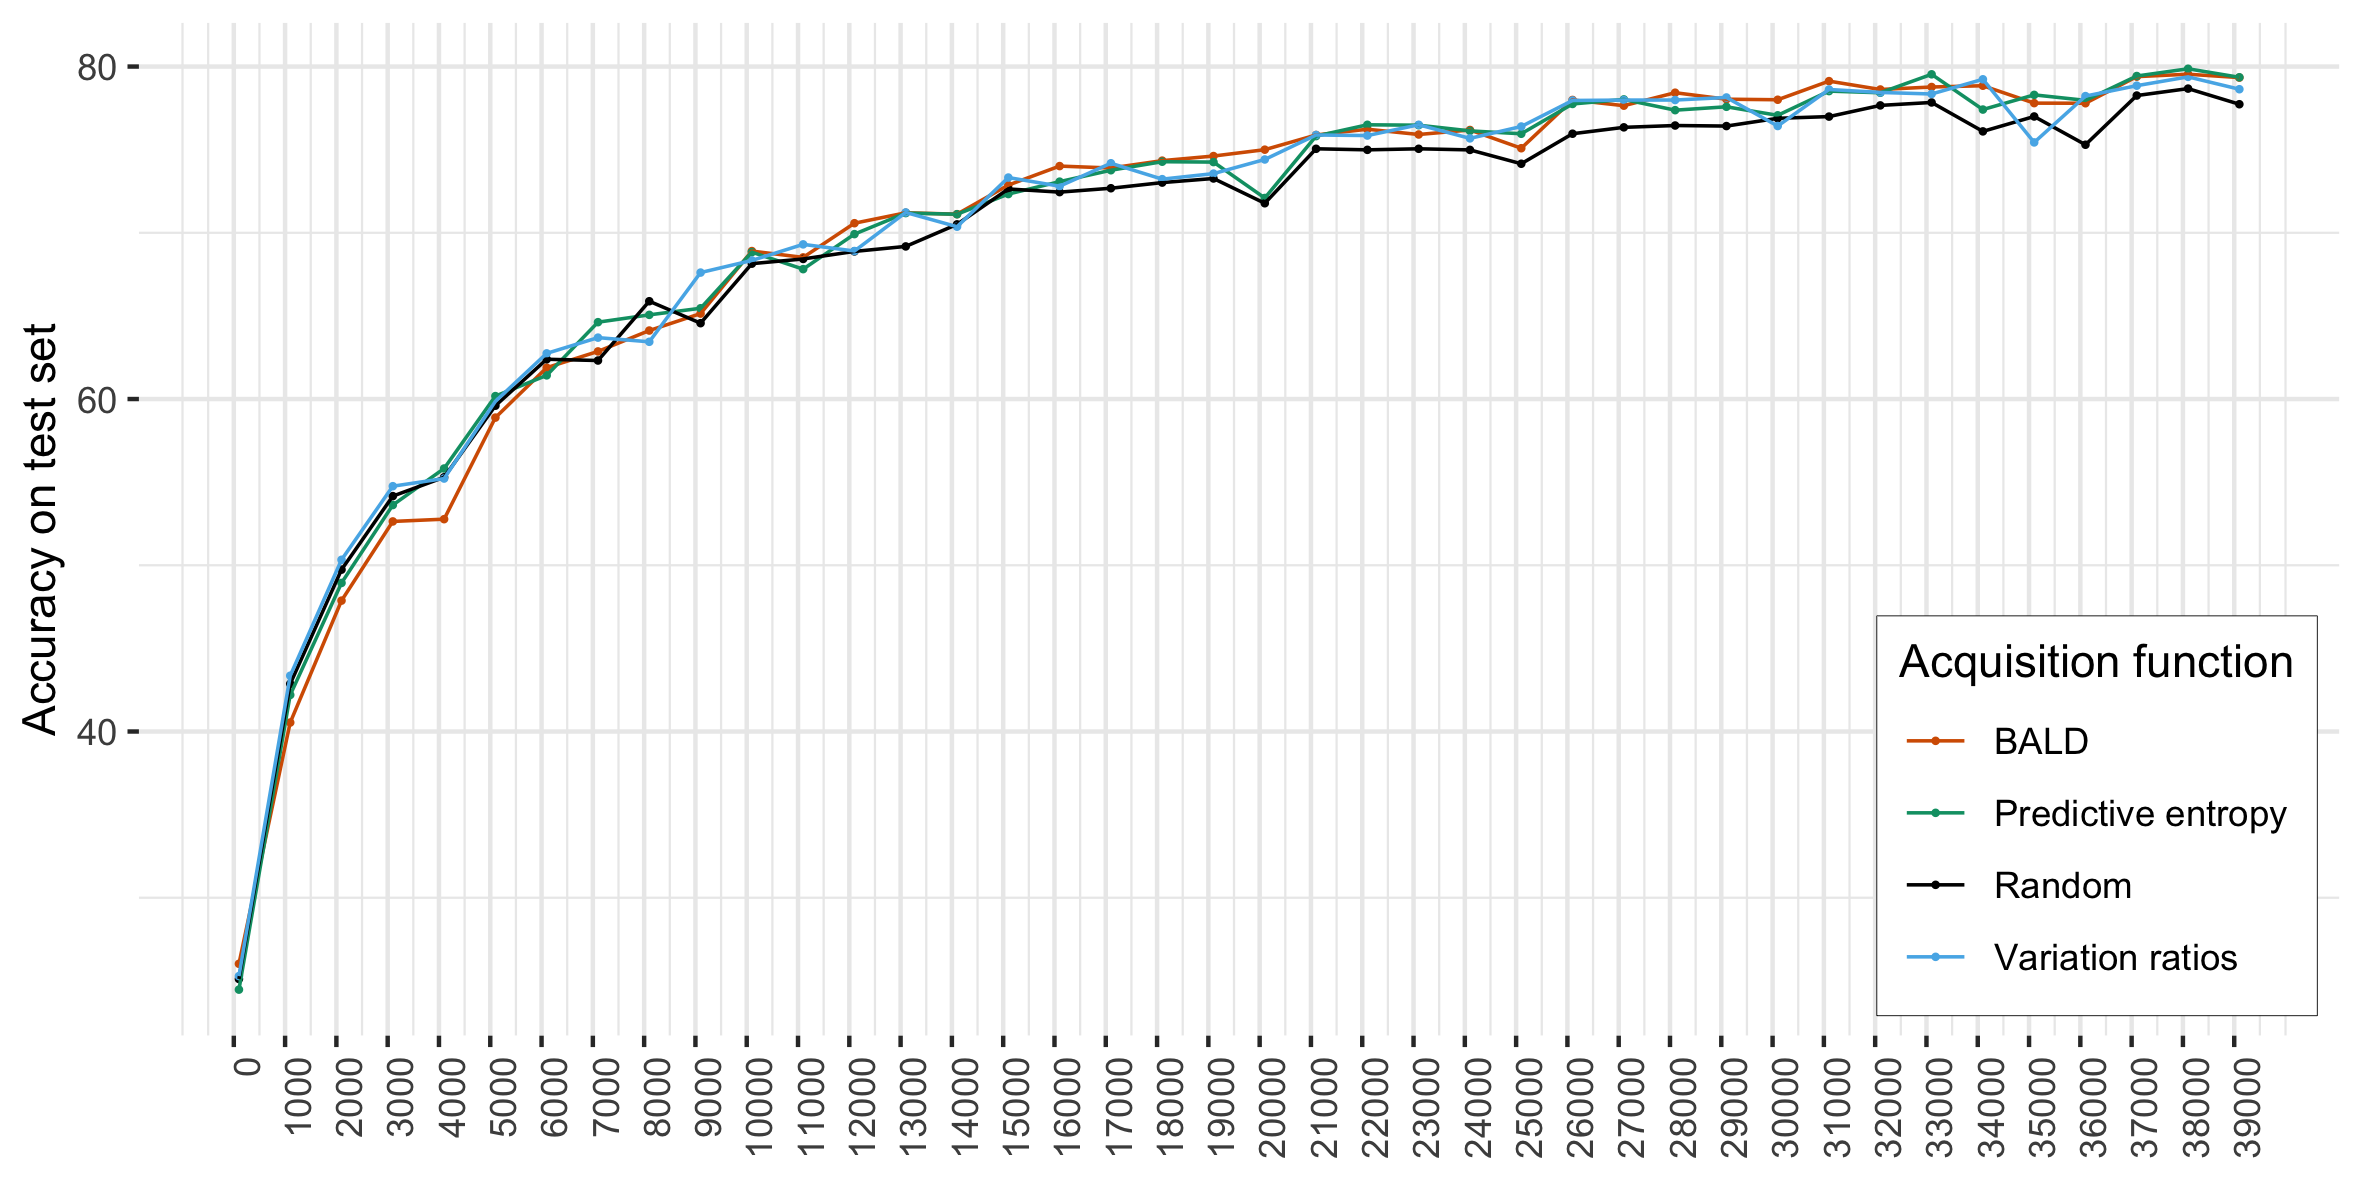
\includegraphics[width=\textwidth]{CIFAR10_accuracies_bayesian}
    \caption{Accuracy of models in each acquisition step in the cats and dogs dataset.}
    \label{fig:CIFAR10_accuracies_bayesian}
\end{figure}



\begin{figure}[H]
    \centering
    \subfloat[Our Predictive entropy.]{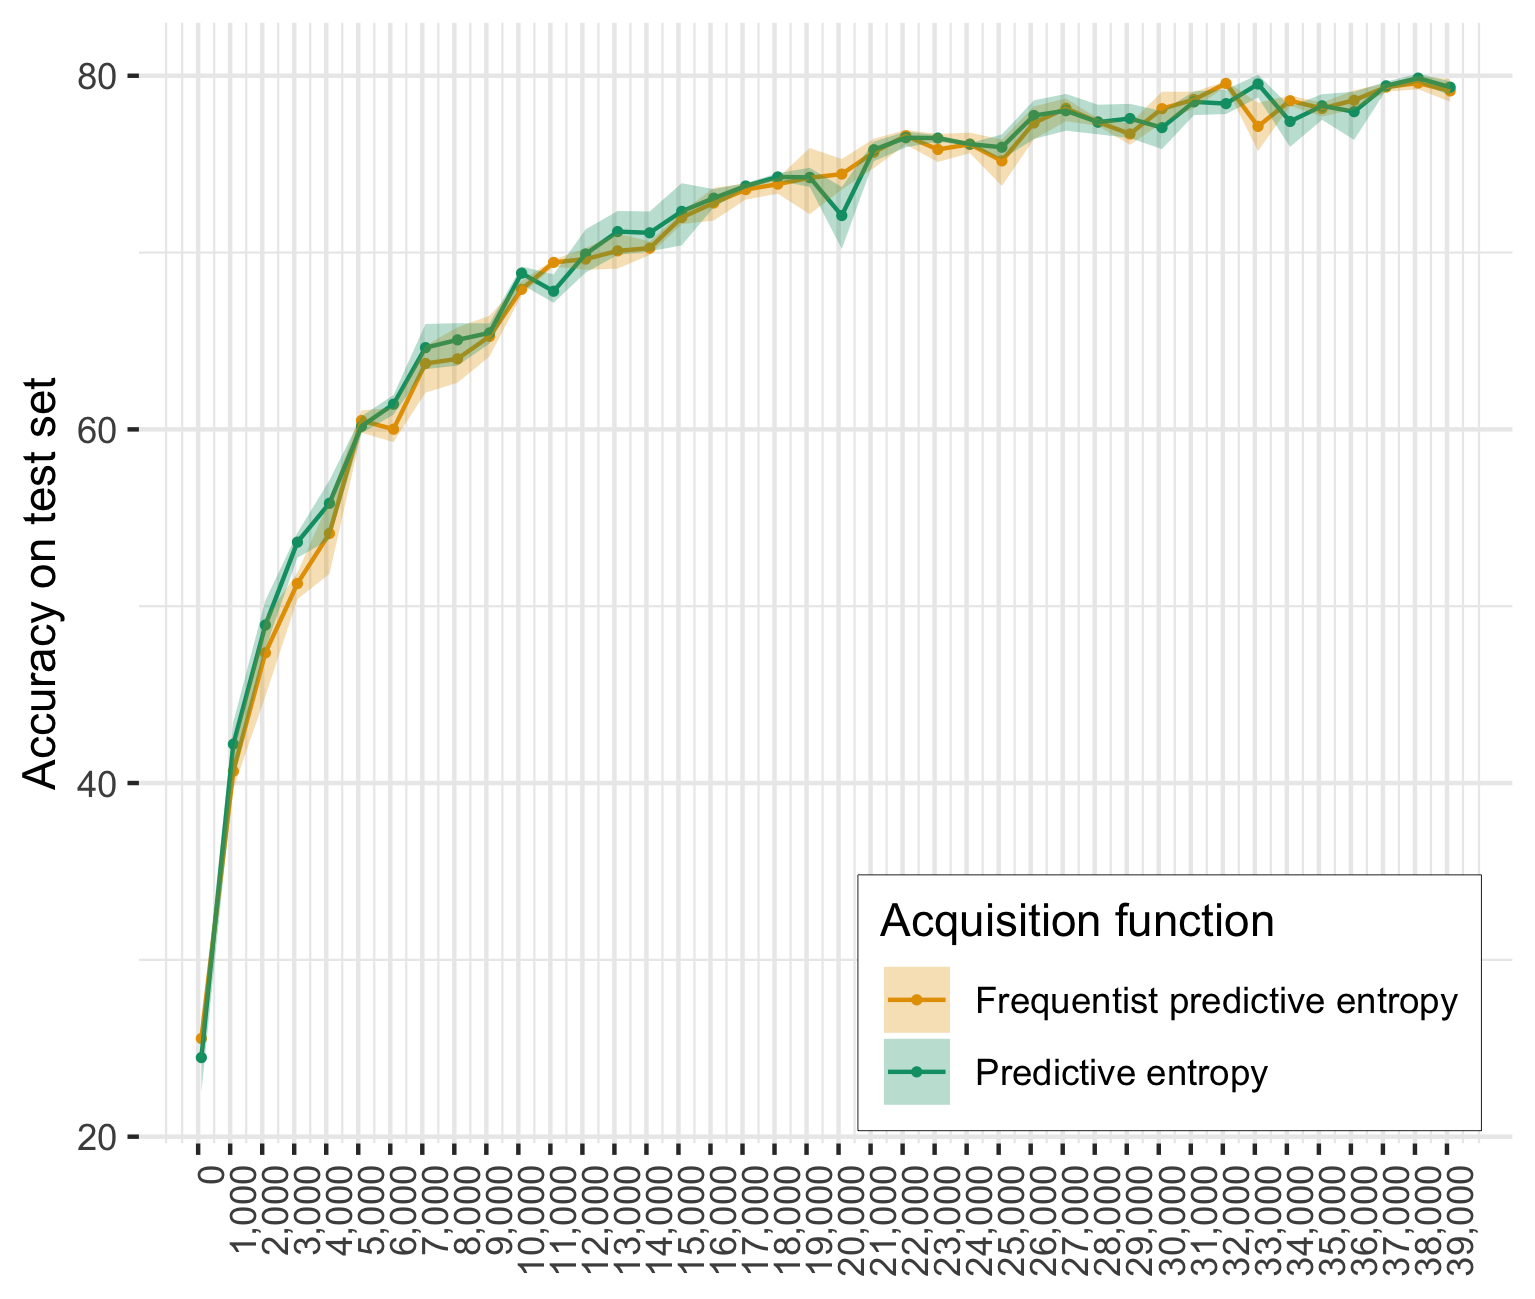
\includegraphics[width=0.5\textwidth]{CIFAR10_accuracies_pred_ent_ribbon}}
    \hfill
    \subfloat[Variation ratios.]{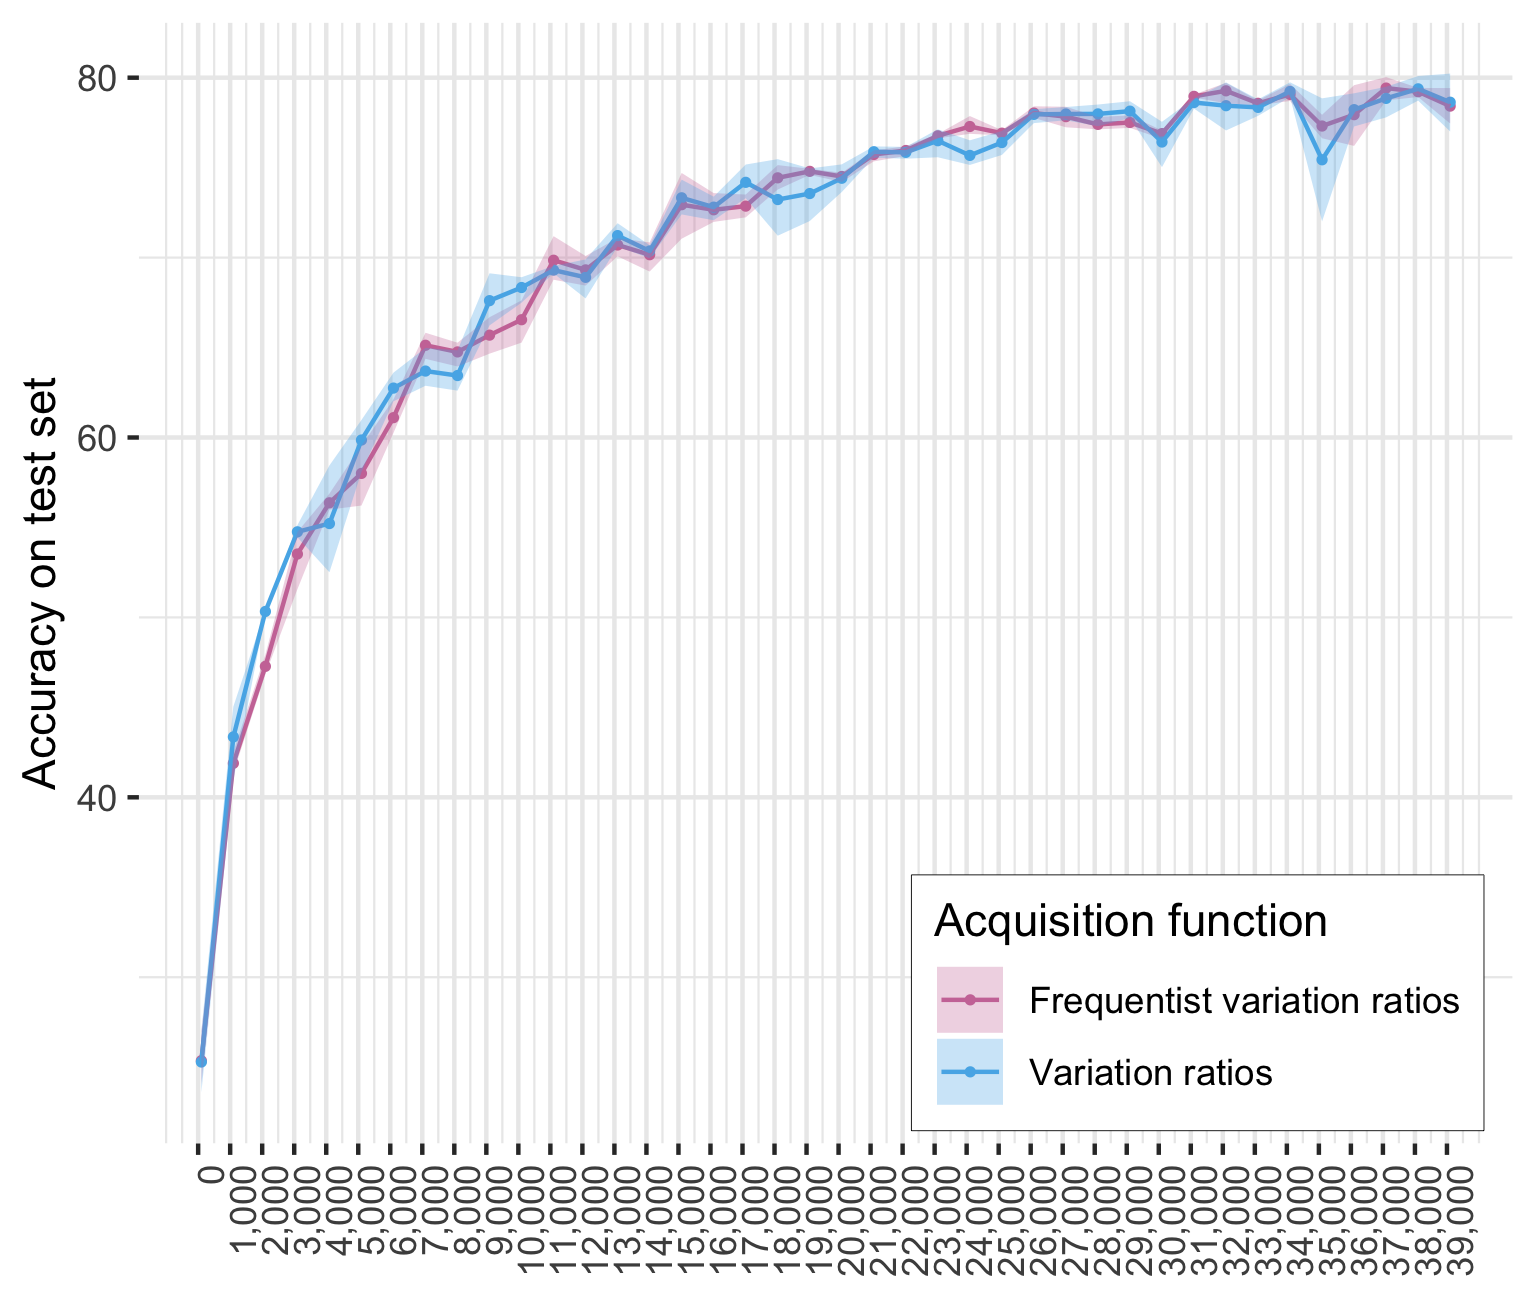
\includegraphics[width=0.5\textwidth]{CIFAR10_accuracies_var_ratios_ribbon}}
    \caption{Accuracy of models in each acquisition step.}
    \label{fig:CIFAR10_bayesian_vs_freq}
\end{figure}



%%%%%%%%%%%%%%%%%%%%%%%%%%%%%%%%%%%%%%%%%%%%%%%%%%%%%%%%%%%%%%
%%%%%%%%%%%%%%%%%%%%%%%%%%%%%%%%%%%%%%%%%%%%%%%%%%%%%%%%%%%%%%
\section{Discussion}
%%%%%%%%%%%%%%%%%%%%%%%%%%%%%%%%%%%%%%%%%%%%%%%%%%%%%%%%%%%%%%
%%%%%%%%%%%%%%%%%%%%%%%%%%%%%%%%%%%%%%%%%%%%%%%%%%%%%%%%%%%%%%


\begin{figure}[H]
    \centering
    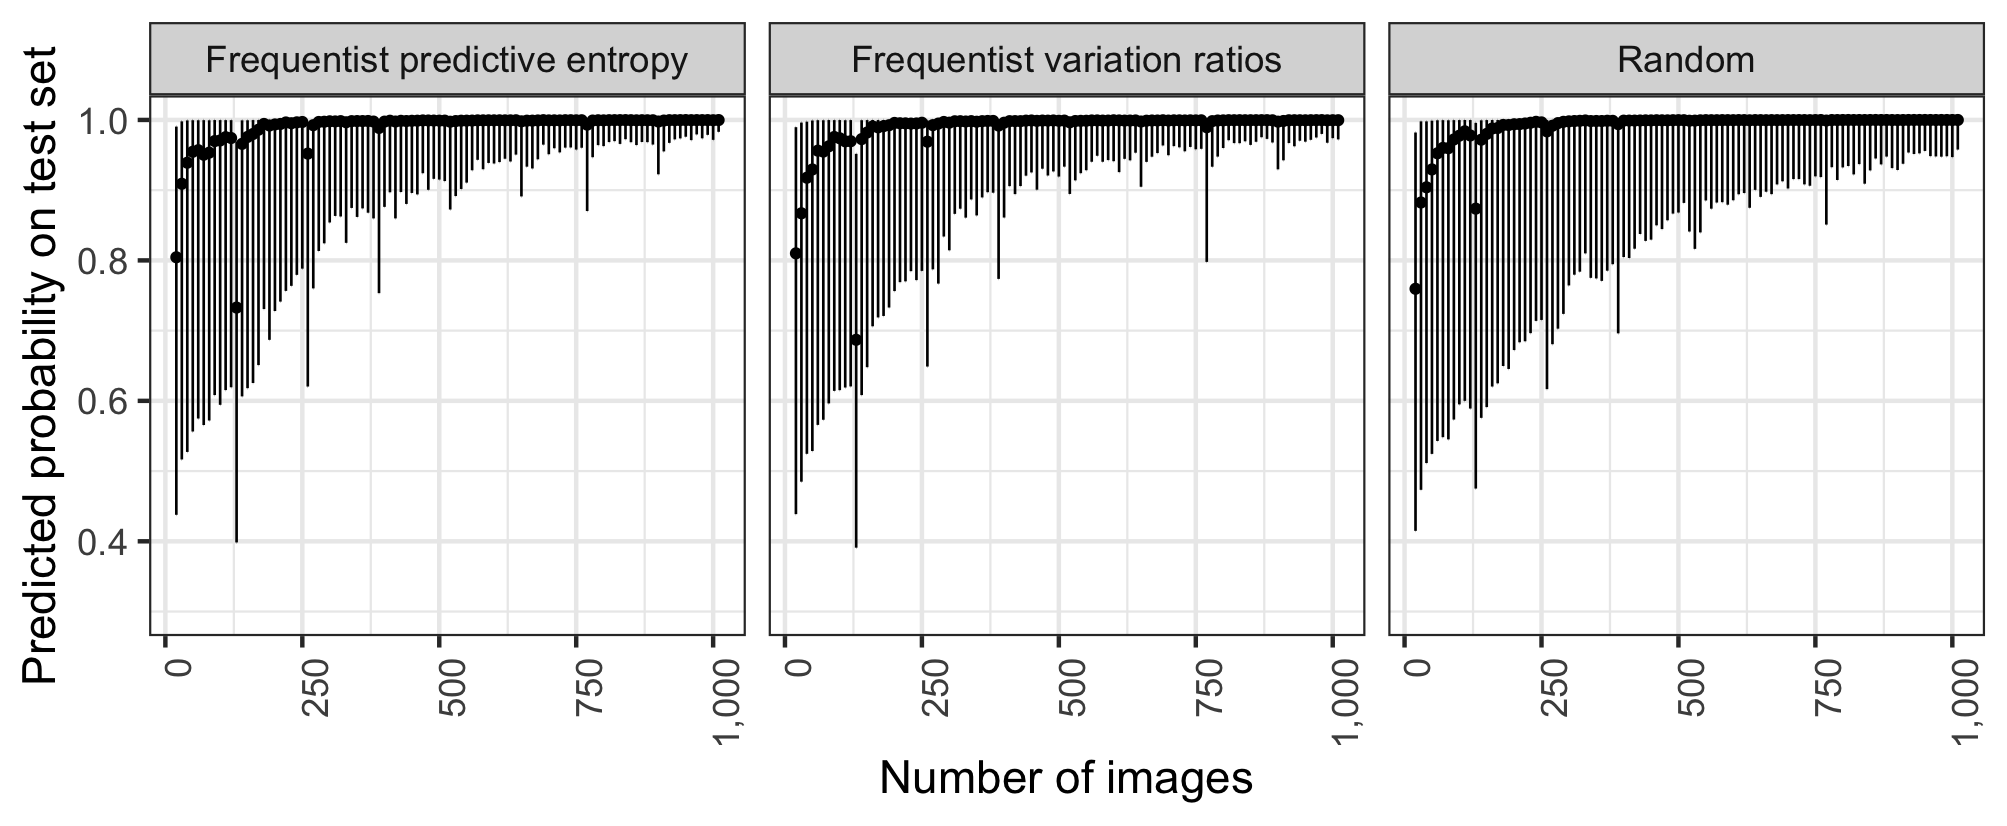
\includegraphics[width=\textwidth]{MNIST_probs_plot}
    \caption{Predicted probabilities in each acquisition iteration for the MNIST dataset.}
    \label{fig:MNIST_probs_plot}
\end{figure}


\begin{figure}[H]
    \centering
    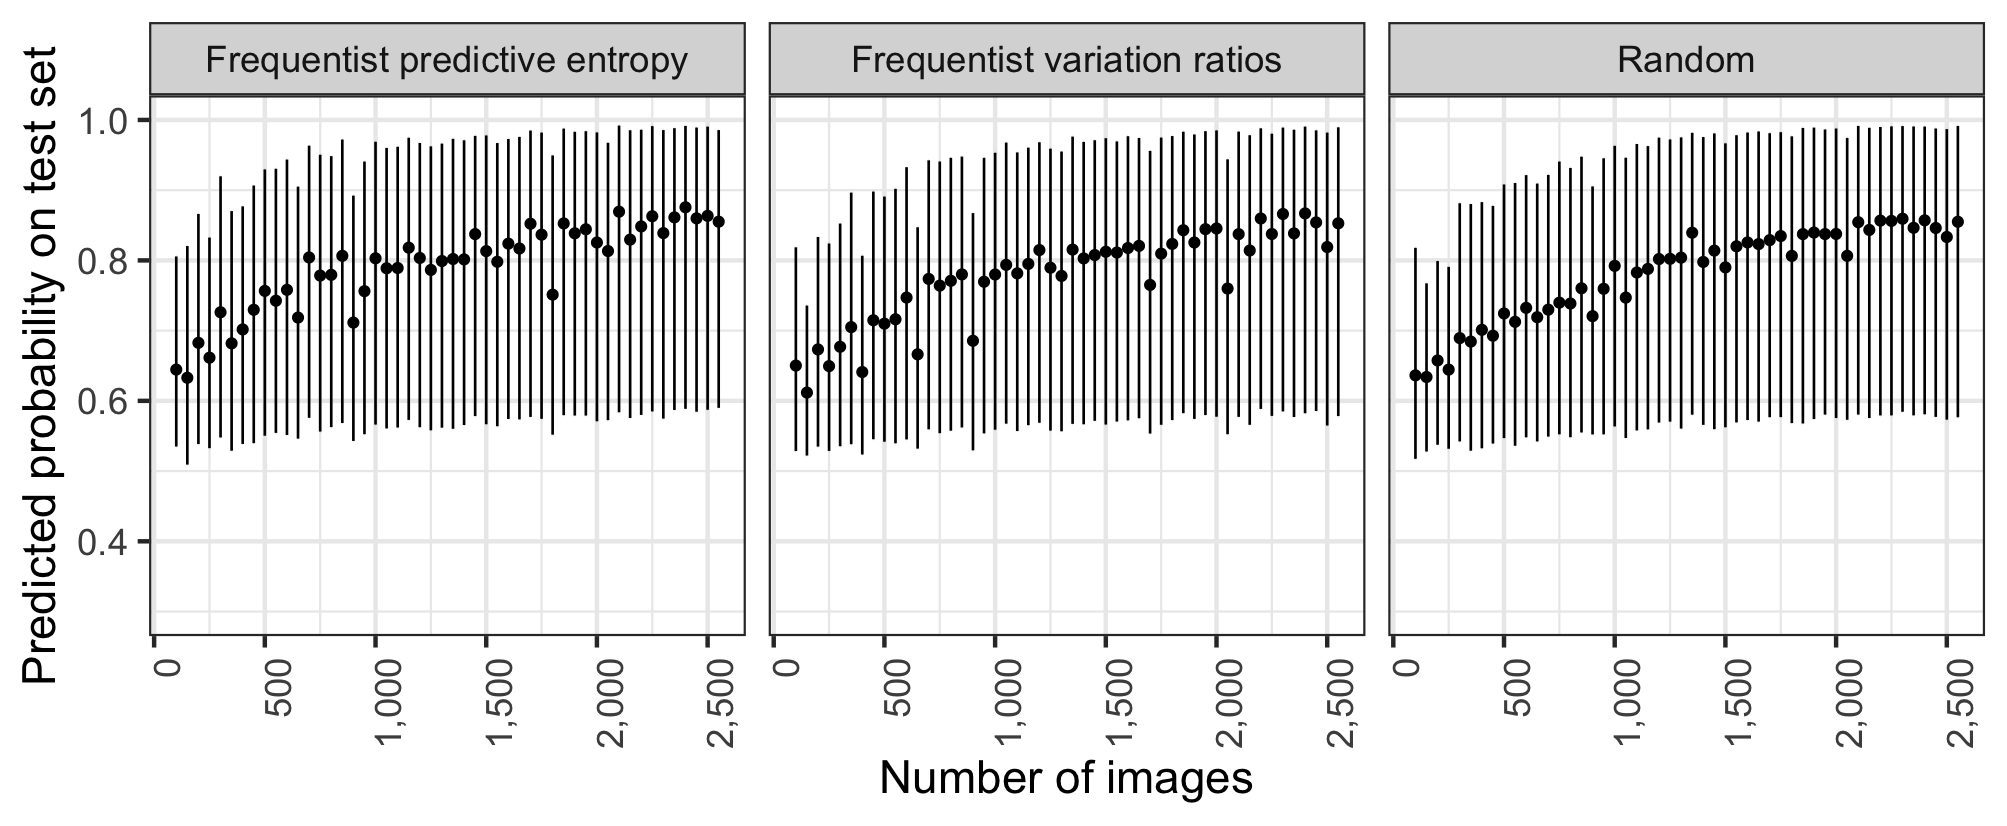
\includegraphics[width=\textwidth]{cats_dogs_probs_plot}
    \caption{Predicted probabilities in each acquisition iteration for the cats and dogs dataset.}
    \label{fig:cats_dogs_probs_plot}
\end{figure}


\begin{figure}[H]
    \centering
    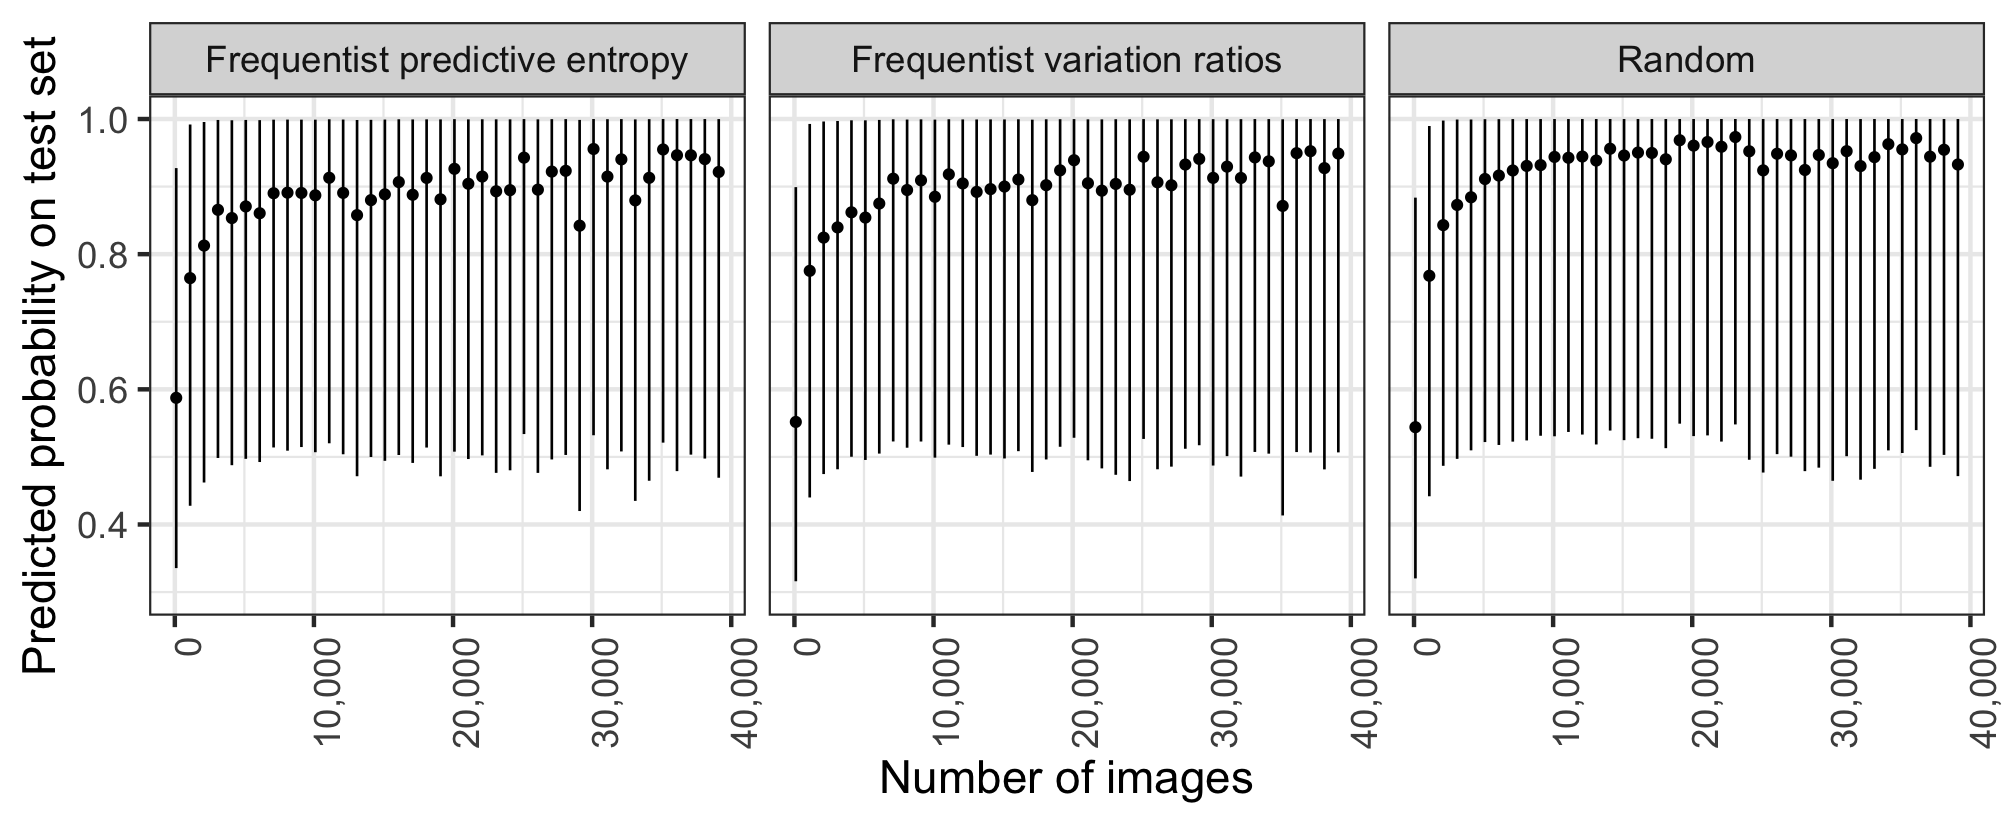
\includegraphics[width=\textwidth]{CIFAR10_probs_plot}
    \caption{Predicted probabilities in each acquisition iteration for the CIFAR10 dataset.}
    \label{fig:CIFAR10_probs_plot}
\end{figure}
